\documentclass{report}
\usepackage{graphicx} % Required for inserting images
\usepackage{}
\usepackage{bm}
%KA packages
\usepackage{tikz}
\usetikzlibrary{automata, arrows.meta, positioning}
\usepackage{pxfonts}
\usepackage{afterpage}
\newcommand\blankpage{%
    \null
    \thispagestyle{empty}%
    \addtocounter{page}{-1}%
    \newpage}
\usepackage[T1]{fontenc}
\usepackage{geometry}
\usepackage{titlesec}
\usepackage{titletoc}
\usepackage{blindtext}

 
%\usepackage{indentfirst}

\usepackage{hyperref}


\title{UTEI}
\author{Urban Tadeáš, Cichra Radek }
\date{August 2023}

\begin{document}


\maketitle

\afterpage{\blankpage}

\chapter*{Předmluva}
Vážení studenti,\newline
na základě našich vlastních zkušeností jsme pro Vás připravili tuto učební pomůcku, která je psána především pro praktické využití. Text si nečiní ambice obsáhnout celou problematiku automatů a proto jej, prosím, považujte za jeden, nikoli však jediný, zdroj informací nutných k přípravě na zkoušku z UTEI.\newline 
Děkujeme.
\newline
\newline
Přejeme Vám hodně úspěchů ve studiu!
\newline


\renewcommand{\contentsname}{Obsah}
\tableofcontents


%PDF 1 ===========================================================================%
\setcounter{chapter}{1}
\chapter*{Formální abeceda, Formální jazyk, Práce s formálními jazyky}
\addcontentsline{toc}{chapter}{Formální abeceda, Formální jazyk, Práce s formálními jazyky}
\section{(Formální) abeceda}

\subsection*{Definice}
Jako abecedu definujeme \textbf{libovolnou konečnou množinu prvků} $\mathbf{\Sigma}$. \newline
Prvky abecedy nejčastěji nazýváme symboly, znaky, nebo písmena.
\subsection*{Příklady}
\begin{itemize}
    \item[] $\mathbf{{\Sigma}_{bin} = \{ 0,1 \}}$  $\mid$ abeceda binární soustavy
    \item[] $\mathbf{{\Sigma}_{dec} = \{ 0,1,2,3,4,5,6,7,8,9 \}}$  $\mid$ abeceda desítkové soustavy
    %~ v ASCII%
    \item[] $\mathbf{{\Sigma}_{ASCII} = \{  <SPACE>, !, '', \#, \$, \%, … … … , y, z, \{,\;, \}, <DEL>\}}$  $\mid$ abeceda printable znaků ASCII standardu 
\end{itemize}

\section{Slovo}
\subsection*{Definice}
Slovo \textbf{w} nad abecedou $\mathbf{\Sigma}$ definujeme jako libovolnou konečnou posloupnost znaků z abecedy $\mathbf{\Sigma}$.
Znaky ve slově se mohou opakovat. \\ \\
  Slovo neobsahující žádný znak nazveme \textbf{prázdné slovo}, dle konvence označované symbolem $\mathbf{\varepsilon}$.


\subsection*{Příklady}
Pro $\mathbf{\Sigma = \{0,1\}}$ je slovo $\mathbf{w = 100110}$ slovem nad $\mathbf{\Sigma}$ (pro všechny znaky ve \textbf{w} platí, že $\in\mathbf{\Sigma})$.
\\ \\
Naopak pro $\mathbf{\Sigma = \{0,1\}}$ slovo $\mathbf{u = 38 }$(w v desítkové soustavě) není slovem nad $\mathbf{\Sigma}$.

\section{Konvence značení abeced a slov}
\begin{description}
    \item[\fbox{$\Sigma^{*}$}] množina všech slov nad abecedou $\Sigma$  $\mid$ $\Sigma^{*}$ = \{ w $\mid$ w je slovem nad  $\Sigma$ \}
    \item[\fbox{$\Sigma^{+}$}]  množina všech slov and abecedou $\Sigma$ bez prázdného slova ($\Sigma^{*}\backslash \{\varepsilon\}$)
    \item[\fbox{$\mid$w$\mid$}] délka slova $\mathbf{w}$
    \item[\fbox{$\mid$w$\mid_x$}] počet výskytů znaku \textbf{x} ve slově \textbf{w}
    \item[\fbox{$\mathbf{a^{n}}$}] kompaktní zápis řetězce opakujících se znaků za sebou $\mid$  $\mathbf{a^{3} = aaa}$
\end{description}

\section{Operace se slovy}
\subsection*{Zřezězení}
Zřetězení slov $\mathbf{u = u_1u_2…u_{n}}$ a $\mathbf{v = v_1v_2…v_{m}}$ značíme \textbf{u.v} (nebo jen \textbf{uv}) a definujeme jako připojení \textbf{v} za \textbf{u}, 
neboli $\mathbf{u.v = uv = u_1u_2…u_n v_1v_2…v_m}$.
\\ \\  Logicky platí, že $\mid$u$\mid$  +  $\mid$v$\mid$ = $\mid$uv$\mid$.
Zřetězení je asociativní.


\section{Prefix, Sufix, Podslovo}

\begin{description}

%TODO DODELAT BOLD 
    \item[\fbox{Prefix}] slovo \textbf{t} je prefixem slova \textbf{z}, pokud platí, že existuje slovo \textbf{u} takové, že platí $\mathbf{z = t.u}$. Pokud z = FJFI, pak například t = FJ je prefix, protože existuje u = FI
    \item[\fbox{Sufix}] slovo t je sufixem slova z, pokud platí, že existuje slovo u takové, že platí z = u.t Pokud z = FJFI, pak například t = FI je sufix, protože existuje u = FJ
    \item[\fbox{Podslovo}] slovo t je podslovem slova z, pokud platí, že existuje slovo u a slovo v takové, že platí z = utv
Pokud z = FJFI, pak například t = JF je podslovo, protože existují u = F a v = I

\end{description}

\section{Jazyk}

\subsection*{Definice}
Jazyk \textbf{L} nad abecedou $\mathbf{\Sigma}$ je libovolná podmnožina slov nad $\mathbf{\Sigma}$.(neboli $\mathbf{L \subseteq \Sigma^*}$)
\subsection*{Příklady}
Nechť \textbf{L} je jazykem všech neprázdných slov délky přesně 3 znaky nad abecedou $\mathbf{\Sigma = \{0,1\}}$. Pak \textbf{L} bude obsahovat všechny permutace čísel obsahujících pouze čísla \textbf{0} a \textbf{1} o délce právě 3 cifer $\Rightarrow$ $\mathbf{L=\{000,111,011,001,100,110,101,010\}}$.
\pagebreak
\section{Operace s jazyky}
\subsection*{Definice}
Hlavní 2 operace, se kterými se v kontextu jazyků při příkladech setkáme, jsou:
\vspace{0.4cm}    
\hrule
\vspace{0.1cm}
\begin{description}

   \item[\fbox{\textbf{Zřetězení}}] Zřetězení jazyků \textbf{K} a \textbf{L} značíme \textbf{KL} a definujeme jako jazyk všech slov \textbf{w} tvaru $\mathbf{w = uv}$, kde $\mathbf{u \in K}$ a $\mathbf{v \in L}$. \\$\Rightarrow \mathbf{KL = \{ uv \mid (u\in K)\land(v\in L) \}}$
   \item[\fbox{\textbf{Iterace}}] Iteraci jazyka \textbf{L} značíme $\mathbf{L^*}$ a definujeme jako rekurentí zřetězení \textbf{L} se sebou $\Rightarrow \mathbf{\varepsilon,L,LL,LLL,...,L^n}$.

\end{description}
\vspace{0.1cm}    
\hrule
\vspace{0.4cm} 

\subsection*{Příklady}

Pro jazyky $\mathbf{K=\{a,ab,\varepsilon\}}$ a $\mathbf{L=\{1,3}\}$ bude $\mathbf{KL=\{a1,a3,ab1,ab3,1,3\}}$
\\ \\
Pro jazyk $\mathbf{L = \{1,0\}}$ bude $\mathbf{L^* = \{\varepsilon, 0,1,00,11,01,10,000,111,001,011,...\}}
\\ \Rightarrow$ nekonečná (ale spočetná) množina všech kladných celých čísel vyjádřených ve dvojkové soustavě.
%PDF 1 KONEC ========================================================================%
%PDF 2-3 KONECNE AUTOMATY===============================================%
\setcounter{chapter}{2}
\setcounter{section}{0}
\chapter*{Konečné automaty}
\addcontentsline{toc}{chapter}{Konečné automaty}
\section{Konečný automat}

\subsection*{Definice}
    Konečný automat (značíme KA) definujeme jako uspořádanou pětici $\mathbf{A = \{Q,\Sigma,\delta,q_0,F\}}$, kde:
\vspace{0.4cm}    
\hrule
\vspace{0.1cm}
    \begin{description}
        \item[\fbox{Q}] Konečná neprázdná množina stavů
        \item[\fbox{$\mathbf{\Sigma}$}] Vstupní abeceda
        \item[\fbox{$\mathbf{\delta}$}] Přechodová funkce pro dané znaky abecedy mezi stavy $\mid$ $\mathbf{Q \times \Sigma \rightarrow Q}$
        \item[\fbox{$\mathbf{q_0}$}] Počáteční stav KA $\mid$ $\mathbf{q_0 \in Q}$
        \item[\fbox{F}] množina koncových stavů KA $\mid$ $\mathbf{F \subseteq Q}$
    \end{description}
\vspace{0.1cm}    
\hrule
\vspace{0.4cm}  
KA může "zpracovat" slovo $\mathbf{v \in \Sigma^*}$ a následně rozhodnout, jestli toto slovo přijímá, nebo ne.
    \\ \\
     Zpracováním slova se rozumí to, že automat začné ve svém počátečním stavu $\mathbf{q_0}$ a čte jednotlivé znaky vstupního slova, přičemž se řídí přechodovou funkcí $\delta$. Přechodová funkce definuje v každém stavu přechod do dalšího stavu podle toho, jaký znak zrovna čte.
     \\ \\ 
     Pokud se po zpracování celého slova automat nachází v nějakém stavu z množiny koncových stavů ($\mathbf{\in F}$) $\mathbf{\rightarrow}$ KA slovo \textbf{akceptuje}. V opačném případě ($\mathbf{\notin F}$) slovo \textbf{neakceptuje}.

\section{Graf KA (Stavový diagram)}
\subsection*{Definice}
Pro intuitivnější vyobrazení a vyjádření struktury a funkce KA používáme \textbf{stavový diagram}. Ten ukazuje množinu stavů \textbf{Q} jako vrcholy grafu a členy přechodové funkce $\delta$ jako hrany mezi vrcholy. Počáteční stav $\mathbf{q_0}$ je vyobrazen jako vrchol, do kterého směřuje hrana z prázdna. Koncové stavy množiny \textbf{F} jsou vrcholy grafu v kruhu (někdy také vrcholy, ze kterých vychází hrana do prázdna).
\subsection*{Příklad}
Následuje příklad stavového diagramu KA, jehož abeceda je $\mathbf{\Sigma = \{0,1\}}$. Stav $\mathbf{q_0}$ je vstupní stav. Stavy $\mathbf{q_3}$ a $\mathbf{q_4}$ ukazují dva nejčastější způsoby vyobrazení stavů koncových $\in \mathbf{F}$.\\ \\


\begin{center}
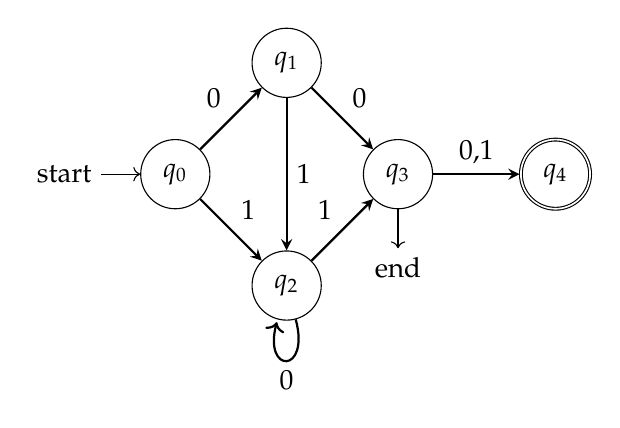
\begin{tikzpicture} [node distance = 2cm , on grid, auto]

    \node (q0) [state, initial] {$q_0$};
    \node (q1) [state, above right = of q0] {$q_1$};
    \node (q2) [state, below right = of q0] {$q_2$};
    \node (q3) [state, accepting below, accepting text=end, below right = of q1] {$q_3$};
    \node (q4) [state, accepting, right = of q3] {$q_4$};

    \path [-stealth, thick] (q0) edge node {0} (q1);
    \path [-stealth, thick] (q1) edge node {1} (q2);
    \path [-stealth, thick] (q0) edge node {1} (q2);
    \path [-stealth, thick] (q2) edge [loop below] node {0}();
    \path [-stealth, thick] (q2) edge node {1} (q3);
    \path [-stealth, thick] (q1) edge node {0} (q3);\
    \path [-stealth, thick] (q3) edge node {0,1} (q4);
    
        
\end{tikzpicture}
\end{center}

\section{Deterministický a nedeterminisitcký KA (DKA a NDKA)}
\subsection*{Definice}
Podle požadavků kladených na přechodovou funkci $\delta$ můžeme rozdělit KA na :

\vspace{0.4cm}    
\hrule
\vspace{0.1cm}
\begin{description}
    \item[\fbox{\textbf{Deterministický KA}}] Z každého stavu by měl být definován právě jeden přechod pro každý znak ze vstupní abecedy $\mathbf{\Sigma}$. 
    
    Toto často striktně neplatí kvůli potenciálně obrovskému množství ($\mathbf{Q . \Sigma}$) hran ve statovém diagramu. Tento problém se někdy řeší tzv. \textbf{error} nebo \textbf{trap stavem}, do kterého automat přejde, jakmile nemá definovaný přechod pro daný znak z daného stavu.

    $\Rightarrow$ pro dané slovo $\mathbf{v \in \Sigma^*}$ existuje právě jedna cesta průchodu stavovým diagramem automatu určená jeho znaky (proto deterministický).
    
    \item[\fbox{\textbf{Nedeterministický KA}}] Z každého stavu může existovat více než jeden přechod pro daný znak.

    $\Rightarrow$ pro dané slovo $\mathbf{v \in \Sigma^*}$ může existovat více možných průchodů a ne všechna musí skončit v nějákém koncovém stavu.

    
    $\Rightarrow$ pro NDKA platí, že slovo akceptuje $\iff$ existuje minimálně jeden průchod stavovým grafem končící v nějakém koncovém stavu.
\end{description}
\vspace{0.1cm}    
\hrule
\vspace{0.4cm} 

\section{Jazyk akceptovaný automatem}
\subsection*{Definice}
Jazyk automatu \textbf{A} definujeme jako množinu všech slov, která automat akceptuje, neboli $\mathbf{L(A) = \{ v \mid (v \in \Sigma^*) \land }$(\textbf{A akceptuje v})$\mathbf{ \}}$.

\section{Ekvivalence automatů}
\subsection*{Definice}
Automaty \textbf{A} a \textbf{B} jsou ekvivalentní, pokud akceptují právě stejný jazyk ($\mathbf{L(A) = L(B)}$).
\\ \\
Platí, že \textbf{libovolný NDKA lze převést na ekvivalentní DKA}.

\subsection*{Příklad}
Následující automaty jsou ekvivalentní ($\mathbf{L(A) = L(B) = \{ab^na\}}$): 

\vspace{0.1cm}    
\hrule
\vspace{0.4cm} 
\begin{center}
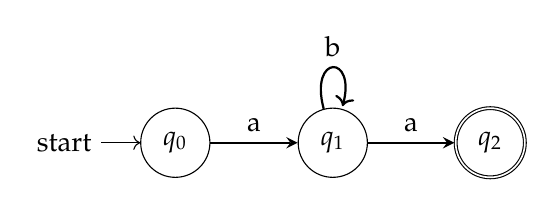
\begin{tikzpicture} [node distance = 2cm , on grid, auto]
    \node (q0) [initial, state] {$q_0$};
    \node (q1) [state, right = of q0] {$q_1$};
    \node (q2) [state, right = of q1, accepting] {$q_2$};

    \path [-stealth, thick] (q0) edge node {a} (q1);
    \path [-stealth, thick] (q1) edge [loop above] node {b} ();
    \path [-stealth, thick] (q1) edge node {a} (q2);
\end{tikzpicture}
\\ \\ 
\vspace{1 cm} 
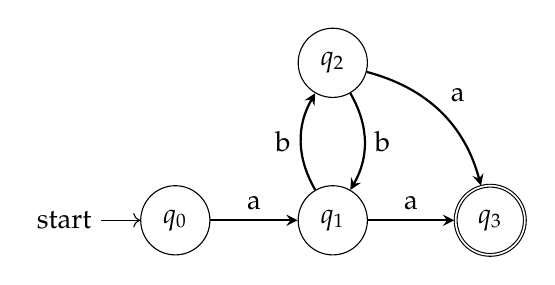
\begin{tikzpicture} [node distance = 2cm , on grid, auto]
     \node (q0) [initial, state] {$q_0$};
    \node (q1) [state, right = of q0] {$q_1$};
    \node (q2) [state, above = of q1] {$q_2$};
    \node (q3) [state, right = of q1, accepting] {$q_3$};

    \path [-stealth, thick] (q0) edge node {a} (q1);
    \path [-stealth, thick] (q1) edge [bend left] node {b} (q2);
    \path [-stealth, thick] (q1) edge  node {a} (q3);
    \path [-stealth, thick] (q2) edge [bend left] node {b} (q1);
    \path [-stealth, thick] (q2) edge [bend left] node [above right] {a} (q3);
    
    
\end{tikzpicture}
\end{center}
\section{Minimální automat}
\subsection*{Definice}
Minimální automat definujeme jako \textbf{automat s nejmenším počtem stavů, který akceptuje daný jazyk}.

\section{Minimalizace}
\subsection*{Definice}
Minimalizace automatu \textbf{A} definujeme jako jeho upravení na ekvivalentní minimální automat $\mathbf{A^{min}}$. Motivace za minimalizací je logicky jednodušší práce s automatem a jeho stavovým diagramem.

\subsection*{Algoritmus minimalizace}
Minimalizace se skládá ze 3 kroků:
\vspace{0.4cm}    
\hrule
\vspace{0.1cm}
\begin{description}
    \item[\fbox{Odstranění nedosažitelných stavů}] Nedosažitelné stavy jsou stavy, do kterých nevedou žádné hrany ve stavovém diagramu $\Rightarrow$ nelze se do nich dostat.
    \item[\fbox{Odstranění nadbytečných stavů}] Nadbytečné stavy jsou stavy, do kterých sice vedou hrany, ale nelze se z nich dostat do koncových stavů diagramu.
    \item[\fbox{Sloučení ekvivalentních stavů}] Ekvivalentní stavy jsou stavy, které generují stejný jazyk, pokud z nich uděláme počáteční stav automatu.
\end{description}
\vspace{0.1cm}    
\hrule
\vspace{0.4cm} 
Nedosažitelné a nadbytečné stavy bývá snadné identifikovat a odstranit (v příkladech, se kterými se setkáme my, jsou zřejmé), proto jejich odstranění v popisu algoritmu přeskočíme.

\subsection*{Nalezení a sloučení ekvivalentních stavů}
Nechť máme automat \textbf{A} popsaný tímto stavovým diagramem:
\begin{center}
\vspace{0.4cm}  
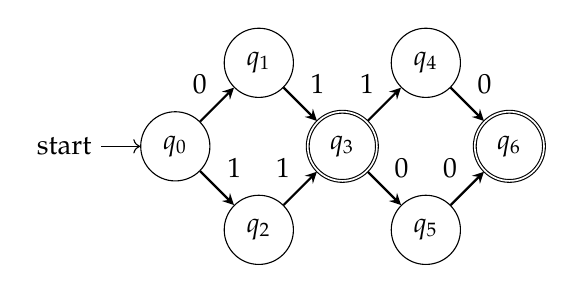
\begin{tikzpicture} [node distance = 1.5cm , on grid, auto]
    \node (q0) [state, initial] {$q_0$};
    \node (q1) [state, above right = of q0] {$q_1$};
    \node (q2) [state, below right = of q0] {$q_2$};
    \node (q3) [state, below right = of q1, accepting] {$q_3$};
    \node (q4) [state, above right = of q3] {$q_4$};
    \node (q5) [state, below right = of q3] {$q_5$};
    \node (q6) [state, below right = of q4, accepting] {$q_6$};

    \path [-stealth, thick] (q0) edge node {0} (q1);
    \path [-stealth, thick] (q0) edge node {1} (q2);
    \path [-stealth, thick] (q1) edge node {1} (q3);
    \path [-stealth, thick] (q2) edge node {1} (q3);
    \path [-stealth, thick] (q3) edge node {1} (q4);
    \path [-stealth, thick] (q3) edge node {0} (q5);
    \path [-stealth, thick] (q5) edge node {0} (q6);
    \path [-stealth, thick] (q4) edge node {0} (q6);
\end{tikzpicture}
\\
\end{center}
\pagebreak
Tento diagram nemá žádné nedosažitelné ani nadbytečné stavy. Pro jeho minimalizaci je tedy třeba pouze nalézt a sloučit ekvivalentní stavy. To uděláme následovně:
\\
\begin{enumerate}
  \item Rozdělíme si množinu stavů \textbf{Q} na 2 množiny $\mathbf{S_1}$ a $\mathbf{S_2}$, kde $\mathbf{S_1=F}$ a $\mathbf{S_2=Q\backslash F}$.
  \\
  $\Rightarrow$\\ $\mathbf{S_1=F=\{q_3,q_6\}}$ \\ $\mathbf{S_2=Q\backslash F=\{q_0,q_1,q_2,q_4,q_5\}}$ 
  \item Vytvoříme takzvanou \textbf{tabulku přechodů} $\rightarrow$ tabulka ukazující pro každý přechod z každého stavu, do jakého stavu vede:\\
 \begin{center}
  \begin{tabular}{c|c|c|c}
       \textbf{Množina} & \textbf{Ze stavu} & \textbf{0 vede do} & \textbf{1 vede do} \\
       $\mathbf{S_1}$ & $q_3$ & $q_5$ & $q_4$ \\
       & $q_6$ & \textbf{X} & \textbf{X} \\ \hline
       $\mathbf{S_2}$ & $q_0$ & $q_1$ & $q_2$ \\
       & $q_1$ & \textbf{X} & $q_3$ \\
       & $q_2$ & \textbf{X} & $q_3$ \\
       & $q_4$ & $q_6$ & \textbf{X} \\
       & $q_5$ & $q_6$ & \textbf{X} \\
  \end{tabular}
  \end{center}
  \item V této tabulce nyní upravíme sloupce s přechody $\rightarrow$ místo cílového stavu uvedeme množinu, do které patří:\\
  \begin{center}
  \begin{tabular}{c|c|c|c}
       \textbf{Množina} & \textbf{Ze stavu} & \textbf{0 vede do} & \textbf{1 vede do} \\
       $\mathbf{S_1}$ & $q_3$ & $S_2$ & $S_2$ \\
       & $q_6$ & \textbf{X} & \textbf{X} \\ \hline
       $\mathbf{S_2}$& $q_0$ & $S_2$ & $S_2$ \\
       & $q_1$ & \textbf{X} & $S_1$ \\
       & $q_2$ & \textbf{X} & $S_1$ \\
       & $q_4$ & $S_1$ & \textbf{X} \\
       & $q_5$ & $S_1$ & \textbf{X} \\
  \end{tabular}
  \end{center}
  \item Přerozdělíme stavy do nových množin tak, že dáme dohromady stavy se stejnými množinami ve sloupcích s přechody:\\
  \begin{center}
  \begin{tabular}{c|c|c|c}
       \textbf{Množina} & \textbf{Ze stavu} & \textbf{0 vede do} & \textbf{1 vede do} \\
       $\mathbf{A}$ & $q_3$ & $S_2$ & $S_2$ \\ \hline
       $\mathbf{B}$ & $q_1$ & \textbf{X} & $S_1$ \\
       & $q_2$ & \textbf{X} & $S_1$ \\ \hline
       $\mathbf{C}$ & $q_6$ & \textbf{X} & \textbf{X} \\ \hline
       $\mathbf{D}$ & $q_0$ & $S_2$ & $S_2$ \\ \hline
       $\mathbf{E}$ & $q_4$ & $S_1$ & \textbf{X} \\
       & $q_5$ & $S_1$ & \textbf{X} \\
  \end{tabular}
  \\
  \end{center}
  (Pozn.: stavy $\mathbf{q_3}$ a $\mathbf{q_0}$ nejsou ve stejné množině, protože $\mathbf{q_3}$ je koncový stav, ale $\mathbf{q_0}$ ne)
  \pagebreak
  \item Kroky 2 až 4 opakujeme, dokud lze stavy přerozdělovat do nových množin:\\
  \begin{center}
  \begin{tabular}{c|c|c|c}
       \textbf{Množina} & \textbf{Ze stavu} & \textbf{0 vede do} & \textbf{1 vede do} \\
       $\mathbf{A}$ & $q_3$ & $E$ & $E$ \\ \hline
       $\mathbf{B}$ & $q_1$ & \textbf{X} & $A$ \\
       & $q_2$ & \textbf{X} & $A$ \\ \hline
       $\mathbf{C}$ & $q_6$ & \textbf{X} & \textbf{X} \\ \hline
       $\mathbf{D}$ & $q_0$ & $B$ & $B$ \\ \hline
       $\mathbf{E}$ & $q_4$ & $C$ & \textbf{X} \\
       & $q_5$ & $C$ & \textbf{X} \\
  \end{tabular}
  \\
    \end{center}
  $\Rightarrow$ nevzniklo nové rozdělení
  \item Máme hotovo. Nyní stačí nakreslit stavový diagram dle tabulky se sloučenými stavy:\\ \\
  \begin{center}
  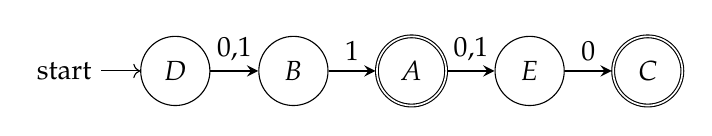
\begin{tikzpicture} [node distance = 1.5cm , on grid, auto]
    \node (D) [state, initial] {$D$};
    \node (B) [state, right = of D] {$B$};
    \node (A) [state, right = of B, accepting] {$A$};
    \node (E) [state, right = of A] {$E$};
    \node (C) [state, right = of E, accepting] {$C$};
    
    \path [-stealth, thick] (D) edge node {0,1} (B);
    \path [-stealth, thick] (B) edge node {1} (A);
    \path [-stealth, thick] (A) edge node {0,1} (E);
    \path [-stealth, thick] (E) edge node {0} (C);

\end{tikzpicture}
\end{center}
\end{enumerate}


\section{$\varepsilon$-přechody}
\subsection*{Definice}
$\varepsilon$-přechod definujeme jako \textbf{přechod mezi stavy, při kterém se ze vstupního slova nečte žádný znak} $\Rightarrow$ Automat může přejít mezi stavy bez čtení znaku ze vstupního slova.
\\ \\
$\varepsilon$-přechodů se můžeme zbavit pomocí $\varepsilon$-uzávěru a nebo při determinizaci.
\subsection*{Příklad}
Následuje stavový diagram automatu \textbf{A}, pro který platí $\mathbf{L(A)=\{a^n \mid n \in \mathbb{N} \}}$\\ \\
\begin{center}
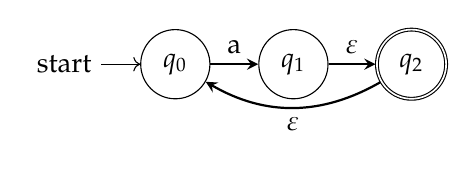
\begin{tikzpicture} [node distance = 1.5cm , on grid, auto]
    \node (q0) [state,initial] {$q_0$};
    \node (q1) [state, right = of q0] {$q_1$};
    \node (q2) [state, accepting, right = of q1] {$q_2$};

    \path [-stealth, thick] (q0) edge node {a} (q1);
    \path [-stealth, thick] (q1) edge node {$\varepsilon$} (q2);
    \path [-stealth, thick] (q2) edge [bend left] node {$\varepsilon$} (q0);
\end{tikzpicture}
\end{center}
\pagebreak
\section{Odstranění $\varepsilon$-přechodů ($\varepsilon$-uzávěr)}
Na příkladě z předchozí části si popíšeme postup vytvoření takzvaných $\varepsilon$-uzávěrů a jejich využití při odstraňování $\varepsilon$-přechodů. Postupujeme následovně:\\
\begin{enumerate}
    \item Pro každý stav automatu definujeme $\varepsilon$-uzávěr $\rightarrow$ \textbf{množina stavů, do kterých se z daného stavu dá dostat bez zpracování znaku vstupního slova} (neboli přes $\varepsilon$-přechody, vždy obsahuje aspoň stav samotný):\\
    \begin{center}
    \begin{tabular}{c|c}
        \textbf{Uzávěr stavu} & \textbf{Stavy v uzávěru} \\ \hline 
         $\varepsilon(q_0)$ & $q_0$  \\
         $\varepsilon(q_1)$ & $q_1, q_2, q_0$ \\
         $\varepsilon(q_2)$ & $q_2, q_0$ \\
    \end{tabular}
    \end{center}
    \item Překreslíme stavový diagram \textbf{BEZ} $\varepsilon$-přechodů:\\ \\
    \begin{center}
    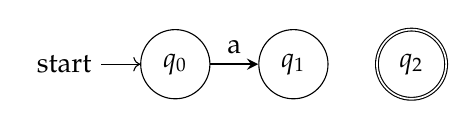
\begin{tikzpicture} [node distance = 1.5cm , on grid, auto]
        \node (q0) [state, initial] {$q_0$};
        \node (q1) [state, right = of q0] {$q_1$};
        \node (q2) [state, right = of q1, accepting] {$q_2$};

        \path [-stealth, thick] (q0) edge node {a} (q1);
    \end{tikzpicture}
    \end{center}
    \item Ke všem stavům diagramu doplníme přechody stavů z jejich $\varepsilon$-uzávěru (ne $\varepsilon$-přechody): \\ \\
    \begin{center}
    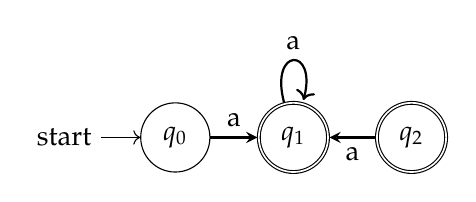
\begin{tikzpicture} [node distance = 1.5cm , on grid, auto]
        \node (q0) [state, initial] {$q_0$};
        \node (q1) [state, right = of q0, accepting] {$q_1$};
        \node (q2) [state, right = of q1, accepting] {$q_2$};

        \path [-stealth, thick] (q0) edge node {a} (q1);
        \path [-stealth, thick] (q1) edge [loop above] node {a} (q1);
        \path [-stealth, thick] (q2) edge node {a} (q1);
    \end{tikzpicture}
    \end{center}
    \\ \\ (Pozn.: $\mathbf{q_1}$ se stává koncovým stavem, neboť v jeho uzávěru byl koncový stav $\mathbf{q_2}$, $\mathbf{q_2}$ je nedosažitelný)
    \\ $\Rightarrow$ Automat je ekvivalentní s:\\ \\
    \begin{center}
    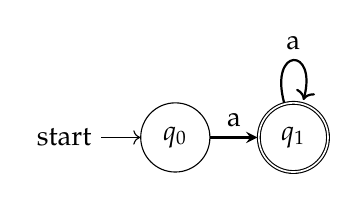
\begin{tikzpicture} [node distance = 1.5cm , on grid, auto]
        \node (q0) [state, initial] {$q_0$};
        \node (q1) [state, right = of q0, accepting] {$q_1$};
        %\node (q2) [state, right = of q1, accepting] {$q_2$};

        \path [-stealth, thick] (q0) edge node {a} (q1);
        \path [-stealth, thick] (q1) edge [loop above] node {a} (q1);
        %\path [-stealth, thick] (q2) edge node {a} (q1);
    \end{tikzpicture}
    \end{center}
    \\ \\ Tím máme hotovo. Stále platí $\mathbf{L(A)=\{a^n \mid n \in \mathbb{N} \}}$.
\end{enumerate}
\section{Determinizace}
\subsection*{Definice}
Determinizace je proces převodu NDKA na ekvivalentní DKA. Postup determinizace si ukážeme na příkladu. Nechť máme následující stavový diagram popisující automat \textbf{A}: \\ \\
\begin{center}
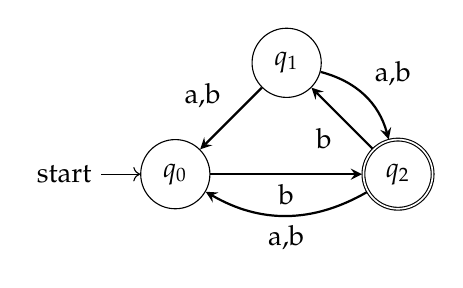
\begin{tikzpicture} [node distance = 2cm, on grid, auto]
    \node (q0) [state, initial] {$q_0$};
    \node (q1) [state, above right = of q0] {$q_1$};
    \node (q2) [state, accepting, below right = of q1] {$q_2$};

    \path[-stealth, thick]( q0) edge node [below] {b}(q2);
    \path[-stealth, thick] (q2) edge node {b}(q1);
    \path[-stealth, thick] (q1) edge node [above left] {a,b}(q0);
    \path[-stealth, thick] (q2) edge [bend left] node {a,b}(q0);
    \path[-stealth, thick] (q1) edge [bend left] node {a,b}(q2);
\end{tikzpicture} \\
\end{center}
Automat \textbf{A} determinizujeme následovně: \\
\begin{enumerate}
    \item Začneme u vstupního stavu a pro každý znak vytvoříme množinu stavů, do kterých se počátečního stavu jejich čtením dostaneme: \\
    \begin{center}
    \begin{tabular}{c|c|c}
         \textbf{Ze stavu}& \textbf{a vede do} & \textbf{b vede do}  \\ \hline
         $q_0$& \textbf{X} & $q_2$ \\
    \end{tabular}\\ \\
    \end{center}
    Zatím tedy máme: \\ \\
    \begin{center}
    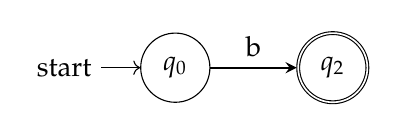
\begin{tikzpicture} [node distance = 2cm, on grid, auto]
        \node (q0) [state,initial] {$q_0$};
        \node (q2) [state, accepting, right= of q0] {$q_2$};

        \path [-stealth, thick] (q0) edge node {b} (q2);
    \end{tikzpicture}
    \end{center}
    \item opakujeme krok 1 pro $\mathbf{q_2}$ a budeme opakovat pro další nově vzniklé stavy, dokud budou vznikat:\\
    \begin{center}
    \begin{tabular}{c|c|c}
         \textbf{Ze stavu}& \textbf{a vede do} & \textbf{b vede do}  \\ \hline
         $q_2$& $q_0$ & $q_0, q_1$ \\
    \end{tabular}\\ \\
    \end{center}
    Doplníme nový stav množiny $\mathbf{\{q_0, q_1\}}$ jako $\mathbf{q_{01}}$ a přechody:\\ \\
    \begin{center}
    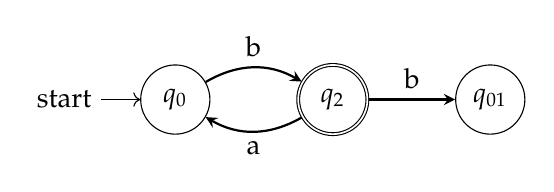
\begin{tikzpicture} [node distance = 2cm, on grid, auto]
        \node (q0) [state,initial] {$q_0$};
        \node (q2) [state, accepting, right= of q0] {$q_2$};
        \node (q01) [state, right = of q2] {$q_{01}$};

        \path [-stealth, thick] (q0) edge [bend left] node {b} (q2);
        \path [-stealth, thick] (q2) edge [bend left] node {a} (q0);
        \path [-stealth, thick] (q2) edge  node            {b} (q01);
    \end{tikzpicture} \\ \\
    \end{center}
    Vznikl nový stav $\Rightarrow$ aplikujeme na něj krok 1 (budeme se koukat na přechody ze všech stavů v množině stavu $\mathbf{q_{01}}$):\\ 
    \begin{center}
    \begin{tabular}{c|c|c}
         \textbf{Ze stavu}& \textbf{a vede do} & \textbf{b vede do}  \\ \hline
         $q_{01}$& $q_0, q_2$ & $q_0, q_2$ \\
    \end{tabular}\\ \\
    \end{center}
    $\Rightarrow$ \\ \\
    \begin{center}
    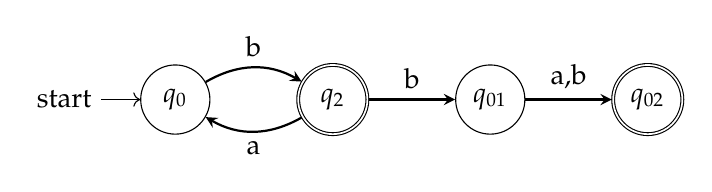
\begin{tikzpicture} [node distance = 2cm, on grid, auto]
        \node (q0) [state,initial] {$q_0$};
        \node (q2) [state, accepting, right= of q0] {$q_2$};
        \node (q01) [state, right = of q2] {$q_{01}$};
        \node (q02) [state, accepting, right = of q01] {$q_{02}$};

        \path [-stealth, thick] (q0) edge [bend left] node {b} (q2);
        \path [-stealth, thick] (q2) edge [bend left] node {a} (q0);
        \path [-stealth, thick] (q2) edge  node            {b} (q01);
        \path [-stealth, thick] (q01)edge node             {a,b}(q02);
    \end{tikzpicture} \\ \\
    \end{center}
    \begin{center}
    \begin{tabular}{c|c|c}
         \textbf{Ze stavu}& \textbf{a vede do} & \textbf{b vede do}  \\ \hline
         $q_{02}$& $q_0$ & $q_0, q_1, q_2$ \\
    \end{tabular}\\ \\ 
    \end{center}
    $\Rightarrow$ \\ \\
    \begin{center}
    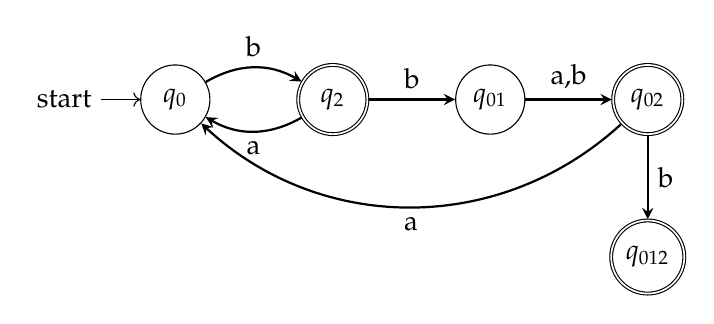
\begin{tikzpicture} [node distance = 2cm, on grid, auto]
        \node (q0) [state,initial] {$q_0$};
        \node (q2) [state, accepting, right= of q0] {$q_2$};
        \node (q01) [state, right = of q2] {$q_{01}$};
        \node (q02) [state, accepting, right = of q01] {$q_{02}$};
        \node (q012) [state, accepting, below = of q02] {$q_{012}$};

        \path [-stealth, thick] (q0) edge [bend left] node {b} (q2);
        \path [-stealth, thick] (q2) edge [bend left] node {a} (q0);
        \path [-stealth, thick] (q2) edge  node            {b} (q01);
        \path [-stealth, thick] (q01)edge node             {a,b}(q02);
        \path [-stealth, thick] (q02)edge [bend left=1.5cm] node {a}(q0);
        \path [-stealth, thick] (q02)edge node {b}(q012);
    \end{tikzpicture}\\ \\
    \end{center}
    \begin{center}
    \begin{tabular}{c|c|c}
         \textbf{Ze stavu}& \textbf{a vede do} & \textbf{b vede do}  \\ \hline
         $q_{012}$& $q_0, q_2$ & $q_0, q_1, q_2$ \\
    \end{tabular}\\ \\ 
    \end{center}
    $\Rightarrow$ \\ \\
    \begin{center}
     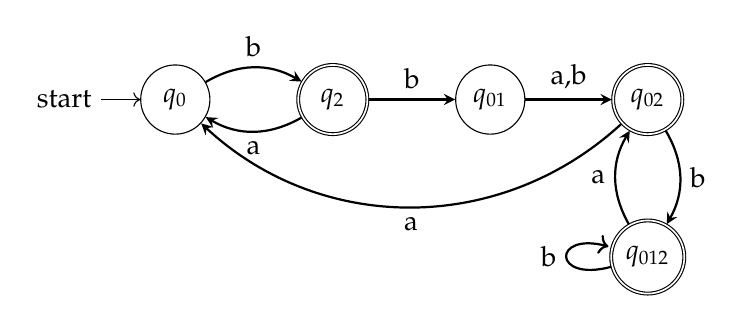
\begin{tikzpicture} [node distance = 2cm, on grid, auto]
        \node (q0) [state,initial] {$q_0$};
        \node (q2) [state, accepting, right= of q0] {$q_2$};
        \node (q01) [state, right = of q2] {$q_{01}$};
        \node (q02) [state, accepting, right = of q01] {$q_{02}$};
        \node (q012) [state, accepting, below = of q02] {$q_{012}$};

        \path [-stealth, thick] (q0) edge [bend left] node {b} (q2);
        \path [-stealth, thick] (q2) edge [bend left] node {a} (q0);
        \path [-stealth, thick] (q2) edge  node            {b} (q01);
        \path [-stealth, thick] (q01)edge node             {a,b}(q02);
        \path [-stealth, thick] (q02)edge [bend left=1.5cm] node {a}(q0);
        \path [-stealth, thick] (q02)edge [bend left] node {b}(q012);
        \path [-stealth, thick] (q012) edge [bend left] node {a} (q02);
        \path [-stealth, thick] (q012) edge [loop left] node {b} (q012);
    \end{tikzpicture}
    \end{center}
    \\ \\ Již nevznikly nové stavy $\Rightarrow$ máme hotovo. Můžeme si všimnout, že automat je nyní opravdu deterministický.
\end{enumerate}
%PDF 2-3 KONEC==========================================================%

%PDF 4 =================================================================%
\setcounter{chapter}{3}
\setcounter{section}{0}
\chapter*{REGEX}
\addcontentsline{toc}{chapter}{REGEX}
\section{Regulární výrazy}
\subsection*{Definice}
Regulární výrazy jsou mocným nástrojem pro popis vzoru nebo určité množiny textových řetězců. Používají se při vyhledávání v textu a vyjádření vzoru, podle kterého řetězec hledat. V kontextu KA jsou regulární výrazy důležité, protože generují takzvané regulární jazyky. Regulární jazyky jsou právě ty stejné jazyky, které mohou generovat a rozpoznávat KA. Tím se pro nás stávají alternativním vyjádřením těchto jazyků. Formálně bychom regulární výraz definovali asi nějak takto:
\\ \\
Nechť existuje abeceda $\mathbf{\Sigma}$. Pak nad $\mathbf{\Sigma}$ definujeme: 
\vspace{0.4cm}    
\hrule
\vspace{0.1cm}
\begin{description}
    \item[\fbox{$\mathbf{\theta}$}] Regulární výraz označující prázdný jazyk
    \item[\fbox{$\varepsilon$}] Regulární výraz označující jazyk \{$\varepsilon$\}
    \item[\fbox{a}] Regulární výraz označující jazyk \{a\}, kde  $\mathbf{a \in \Sigma}$
\end{description}
\vspace{0.1cm}    
\hrule
\vspace{0.4cm}
Nechť existují libovolné regulární výrazy $\alpha$, $\beta$. Pak platí, že i $(\alpha + \beta)$, $(\alpha \cdot \beta)$ a $(\alpha^*)$ jsou regulární výrazy, kde:
\vspace{0.4cm}    
\hrule
\vspace{0.1cm}
\begin{description}
    \item[\fbox{$(\alpha + \beta)$}] Operace sjednocení jazyků $\{\alpha\}$ a $\{\beta\}$ (je asociativní)  \item[\fbox{$(\alpha \cdot \beta)$}] Operace zřetězení $\{\alpha\}$ a $\{\beta\}$ (často bez '$\cdot$' $\rightarrow$ $\alpha\beta$ , je asociativní) 
    \item[\fbox{$(\alpha^*)$}] Operace iterace \{$\alpha$\}
\end{description}
\vspace{0.1cm}    
\hrule
\vspace{0.4cm}
Tyto pravidla nám dovolují popsat celou množinu slov akceptovaných KA (neboli jeho jazyk) popsáním souvislostí ve formátu slov daného jazyka.

\subsection*{Příklady}
\begin{description}
    \item[\fbox{a(a + b)b}] První regulární výraz '\textbf{a}' nám udává, že všechna slova v generovaném jazyce \textbf{J} budou začínat písmenem z jazyka \{a\}. Druhý regulární výraz '\textbf{(a + b)}' udává druhý znak slov v \textbf{J}, a to sice znak ze sjednocení jazyků \{a\} $\cup$ \{b\} $\rightarrow$ \{a,b\}. Analogicky k prvnímu znaku, poslední reg. výraz udává všem slovům z \textbf{J} koncovku \textbf{b}. Dohromady tedy můžeme určit, že všechna slova v \textbf{J} budou mít délku 3 znaků, přičemž jejich prefix je '\textbf{a}', sufix '\textbf{b}' a mezi nimi je znak z jazyka \{a,b\} $\Rightarrow$ Výraz generuje $\mathbf{J = \{aab,abb\}}$.
    \item[\fbox{a(b + $\varepsilon$)c}] Výraz řešíme analogicky k prvnímu příkladu. Rozdíl je různá délka generovaných slov kvůli druhému regulárnímu výrazu '$\mathbf{(b+\varepsilon)}$'. Podle něj budou mít slova generovaného jazyka \textbf{J} na druhé pozici buď znak z jazyka \{b\} nebo \{$\varepsilon$\} $\Rightarrow \mathbf{J = \{abc, a{\varepsilon}c = ac\}}$.
    \item[\fbox{$\mathbf{(a^{*})b(c^{*})}$}] První a poslední reg. výraz jsou iterace jazyků \{a\} a \{c\}. Z definice Iterace jazyka víme, že se jedná o rekurentní zřetězení:\\ 
    $\Rightarrow$ $\mathbf{(a^*) = \{\varepsilon, a, aa, ..., a^n\}}$ a $\mathbf{(c^*)=\{\varepsilon, c, cc, ..., c^n\}}$
    \\ \\ Prostřední výraz '\textbf{b}' je jasný $\Rightarrow$ Jazyk \textbf{J} bude tedy obsahovat slova obsahující prázdný nebo libovolně dlouhý prefix znaků '\textbf{a}' následovaný právě jedním znakem '\textbf{b}' a prázdným nebo libovolně dlouhým sufixem znaků '\textbf{c}' $\Rightarrow$ $\mathbf{J=\{b,ab,bc,aab,abc,bcc,aaab,aabc,abcc,bccc,...\}}$
\end{description}

\section{Převod KA na regulární výraz (eliminace stavů)}
\subsection*{Definice}
Jak bylo již řečeno, existuje vztah mezi jazykem generovaným KA a regulárními výrazy. Platí totiž, že \textbf{oba mohou generovat stejné jazyky} (regulární jazyky). Logicky tedy \textbf{lze KA převést na regulární výraz} (a naopak). \\ \\
Následuje postup převodu KA na regulární výraz skrze takzvanou \textbf{eliminaci stavů}. Tato metoda je spíše intuitivní než algoritmická, ale pro naše účely postačuje. Pro doplnění je vhodné uvést, že stejného lze dosáhnout metodou regulárních rovnic. Postup pro převod KA je následující: \\ \\
\begin{enumerate}
    \item Vytvoříme dva nové stavy -  počáteční $\mathbf{S'}$ a koncový $\mathbf{F'}$.
        \begin{enumerate}
              \item ze stavu $\mathbf{S'}$ povedeme $\varepsilon$-přechody do všech počátečních stavů automatu.
              \item do stavu $\mathbf{F'}$ povedeme $\varepsilon$-přechody ze všech koncových stavů automatu.
        \end{enumerate}
    \item Postupně eliminujeme stavy automatu (v libovolném pořadí) a nahrazujeme zaniklé přechody ekvivalentními reg. výrazy.
    \item Konec převodu nastane, když máme pouze stavy $\mathbf{S'}$ a $\mathbf{F'}$. Hrana mezi těmito stavy bude regulární výraz ekvivalentní s původním KA.
\end{enumerate}
\subsection*{Příklad}
Ukažme si převod automatu \textbf{A} s následujícím stavovým diagramem:\\ \\
\begin{center}
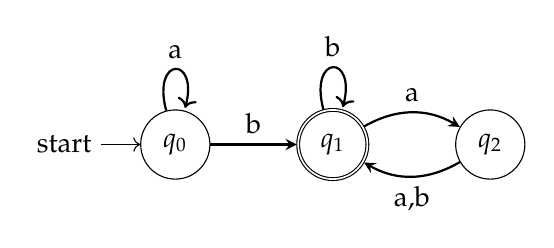
\begin{tikzpicture} [node distance = 2cm, on grid, auto]
        \node (q0) [state,initial] {$q_0$};
        \node (q1) [state,right = of q0, accepting] {$q_1$};
        \node (q2) [state,right = of q1] {$q_2$};

        \path [-stealth, thick] (q0) edge [loop above] node {a} ();
        \path [-stealth, thick] (q0) edge node {b} (q1);
        \path [-stealth, thick] (q1) edge [loop above] node {b} (q1);
        \path [-stealth, thick] (q1) edge [bend left] node {a} (q2);
        \path [-stealth, thick] (q2) edge [bend left] node {a,b} (q1);

    \end{tikzpicture}
    \end{center}
    \\ \\
    
    \begin{enumerate}
        \item Přidáme nové stavy  $\mathbf{S'}$ a $\mathbf{F'}$ a připojíme je:\\ \\
\begin{center}
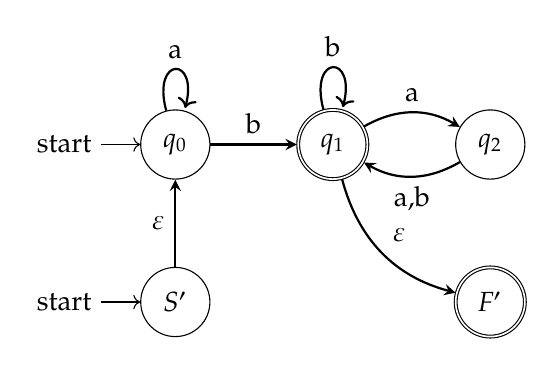
\begin{tikzpicture} [node distance = 2cm, on grid, auto]
        \node (q0) [state,initial] {$q_0$};
        \node (q1) [state,right = of q0, accepting] {$q_1$};
        \node (q2) [state,right = of q1] {$q_2$};
        \node (S') [state, below = of q0, initial] {$S'$};
        \node (F') [state, below = of q2, accepting] {$F'$};

        \path [-stealth, thick] (q0) edge [loop above] node {a} ();
        \path [-stealth, thick] (q0) edge node {b} (q1);
        \path [-stealth, thick] (q1) edge [loop above] node {b} (q1);
        \path [-stealth, thick] (q1) edge [bend left] node {a} (q2);
        \path [-stealth, thick] (q2) edge [bend left] node {a,b} (q1);
        \path[-stealth, thick] (q1) edge [bend right] node{$\varepsilon$}(F');
        \path[-stealth, thick] (S') edge node{$\varepsilon$}(q0);

    \end{tikzpicture}\\ \\
    \end{center}
    \pagebreak
    \item Začneme odstraňovat stavy a nahrazovat hrany. První odstraníme stav $\mathbf{q_0}$ $\rightarrow$ je třeba přidat hrany, které nahradí přechody přes $\mathbf{q_0}$:
    \begin{itemize}
        \item[-] Do $\mathbf{q_0}$ přichází pouze 1 hrana '$\varepsilon$' ze stavu $\mathbf{S'}$.
        \item[-] Z $\mathbf{q_0}$ naopak odchází 2 hrany '$\mathbf{a}$' zpět do $\mathbf{q_0}$ a  '$\mathbf{b}$' do $\mathbf{q_1}$.
    \end{itemize}
    Jelikož do $\mathbf{q_0}$ vede hrana s prázdním slovem '$\varepsilon$' $\rightarrow$ v regulárním výrazu se nijak neprojeví.\\ \\ Zamysleme se nyní nad tím, jak funguje smyčka (hrana $\mathbf{q_0 \rightarrow q_0}$) v automatu. Slovo akceptované automatem \textbf{A} může začínat prázdným nebo libovolně dlouhým sufixem znaků '$\mathbf{a}$', neboť při zpracování 'a' zůstáváme ve stavu $\mathbf{q_0}$ a posouváme se až po přečtení znaku '$\mathbf{b}$' $\rightarrow$ sufix akceptovaných slov může být tvaru $\mathbf{\{\varepsilon, a, aa, ..., a^n\}}$. Nyní je snad zřejmá ekvivalence s reg. výrazem $\mathbf{(a^*)}$.\\ \\ Hrana $\mathbf{q_0 \rightarrow q_1}$ se symbolem '$\mathbf{b}$' je logicky ekvivalentní s regulárním výrazem ($\mathbf{b}$). \\ \\ Po odstranění stavu $\mathbf{q_0}$ tedy spojíme $\mathbf{S' \rightarrow q_1}$ hranou s regulárním výrazem $\mathbf{(a^*)b}$ (pozor na správné pořadí!), čímž pokryjeme jak smyčku $\mathbf{q_0 \rightarrow q_0}$, tak přechod $\mathbf{q_0 \rightarrow q_1}$.\\ \\
\begin{center}
\begin{tikzpicture} [node distance = 2cm, on grid, auto]
        \node (q1) [state,right = of q0, accepting] {$q_1$};
        \node (q2) [state,right = of q1] {$q_2$};
        \node (S') [state, below = of q0, initial] {$S'$};
        \node (F') [state, below = of q2, accepting] {$F'$};

        \path [-stealth, thick] (q1) edge [loop above] node {b} (q1);
        \path [-stealth, thick] (q1) edge [bend left] node {a} (q2);
        \path [-stealth, thick] (q2) edge [bend left] node {a,b} (q1);
        \path[-stealth, thick] (q1) edge [bend right] node{$\varepsilon$}(F');
        \path[-stealth, thick] (S') edge node{$\mathbf{(a^*)b}$}(q1);

    \end{tikzpicture}
    \end{center}
    \item Odstraňujeme stavy, dokud nezůstane pouze $\mathbf{S' \rightarrow F'}$. Odstraníme tedy $\mathbf{q_2}$.
    \begin{itemize}
        \item[-]Do $\mathbf{q_2}$ vede 1 hrana se znakem '$\mathbf{a}$' $\rightarrow \mathbf{(a)}$.
        \item[-]Z $\mathbf{q_2}$ vedou 2 hrany do $\mathbf{q_1}$. Je důležité si uvědomit, že při přechodu $\mathbf{q_2 \rightarrow q_1}$ se přečte jen jeden znak $\rightarrow$ proto $\mathbf{(a + b)}$, ne $\mathbf{(ab)}$.
    \end{itemize} 
    \begin{center}
    \begin{tikzpicture} [node distance = 2cm, on grid, auto]
        \node (q1) [state,right = of q0, accepting] {$q_1$};
        \node (S') [state, below = of q0, initial] {$S'$};
        \node (F') [state, below = of q2, accepting] {$F'$};

        \path [-stealth, thick] (q1) edge [loop above] node {b} (q1);
        \path [-stealth, thick] (q1) edge [loop right] node {$\mathbf{a(a + b)}$} (q1);
        \path[-stealth, thick] (q1) edge [bend right] node{$\varepsilon$}(F');
        \path[-stealth, thick] (S') edge node{$\mathbf{(a^*)b}$}(q1);

    \end{tikzpicture} \\ \\
    \end{center}
    Poslední odstraníme $\mathbf{q_1}$.
    \begin{itemize}
        \item[-] z $\mathbf{q_1}$ vedou 3 hrany, z čehož 2 jsou smyčky a poslední je $\varepsilon$-přechod do $\mathbf{F'}$.
    \end{itemize}
    Jak jsme si již ukázali, smyčky jsou ekvivalentní s iterací $\rightarrow$ máme $\mathbf{(b^*)}$ a $\mathbf{(a(a + b))^*}$. Obě smyčky končí ve stejném stavu $\rightarrow$ akceptovaná slova je mohou nejenom libovolně opakovat, ale také střídat:\\$\rightarrow \mathbf{((b^*)+(a(a+b))^*)^*=(b + (a(a+b)))^*=}$ \fbox{$\mathbf{(b + (aa + ab))^*}$}\\ Vnější iterací výrazu jsme zároveň pokryli možnost $\varepsilon$-přechodu $\mathbf{q_1 \rightarrow F'}$.\\ \\
    \begin{center}
    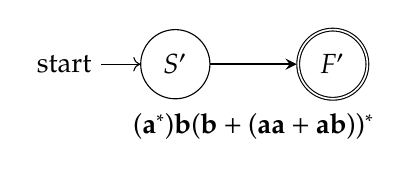
\begin{tikzpicture} [node distance = 2cm, on grid, auto]
        \node (S') [state, initial] {$S'$};
        \node (F') [state, right = of S', accepting] {$F'$};
        \path[-stealth, thick] (S') edge node[below=0.5cm]{$\mathbf{(a^*)b(b + (aa+ab))^*}$}(F');

    \end{tikzpicture} \\ \\ 
    \end{center}
    Tím máme hotovo. Regulární výraz na hraně $\mathbf{S' \rightarrow F'}$ generuje stejný jazyk jako původní automat \textbf{A}.
    \end{enumerate}
    \section{Lemma o vkládání (Pumping lemma)}
    \subsection*{Definice}
    Pro libovolný \textbf{regulární} (akceptovaný konečným automatem) jazyk \textbf{L} existuje nějaké číslo $\mathbf{ p > 0}$ takové, že pro každé slovo $\mathbf{(w \in L)\land({\mid}w{\mid}\ge p)}$ platí následující:
    \begin{enumerate} 
        \item \textbf{w} lze zapsat jako $\mathbf{w=xyz}$ 
        \item pro slova $\mathbf{x,y,z}$ platí, že:
        \begin{enumerate}
            \item $\mathbf{{\mid}xy{\mid}{\leq}p}$
            \item $\mathbf{{\mid}y{\mid}>0}$
            \item $\mathbf{(xy^iz) \in L \mid i\ge0 }$
        \end{enumerate}
    \end{enumerate} 
    Tato definice nám říká, že v regulárním jazyce platí následující:\\ \\
    Dostatečně dlouhé ($\mathbf{{\mid}w{\mid}\ge p}$) slovo z tohoto jazyka můžeme rozdělit takovým způsobem, který nám dovoluje libovolně opakovat jeho část ($\mathbf{y^i}$), aniž by nová slova přestala ležet v daném jazyce.\\ \\
    V praxi \textbf{Pumping lemma používáme při důkazu sporem, kdy chceme ukázat, že nějaký jazyk NENÍ regulární}.
    \subsection*{Příklady}
    Ukažme si lemma na jazyce \textbf{L}, který obsahuje všechna slova nad abecedou $\mathbf{\Sigma=\{0,1\}}$, která končí na '$\mathbf{11}$'. Víme, že \textbf{L} je regulární, protože můžeme celkem snadno navrhnout automat, který ho akceptuje:\\ \\
    \begin{center}
    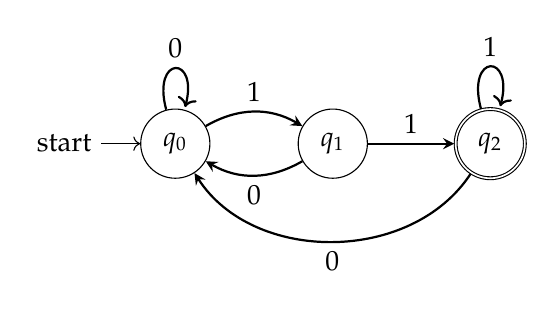
\begin{tikzpicture} [node distance = 2cm, on grid, auto]
        \node (q0) [state,initial] {$q_0$};
        \node (q1) [state,right = of q0] {$q_1$};
        \node (q2) [state,accepting, right= of q1] {$q_2$};

        \path[-stealth, thick](q0) edge [loop above] node {0}(q0);
        \path[-stealth, thick](q0) edge [bend left] node {1}(q1);
        \path[-stealth, thick](q1) edge [bend left] node {0}(q0);
        \path[-stealth, thick](q1) edge node {1}(q2);
        \path[-stealth, thick](q2) edge [bend left=2cm] node {0}(q0);
        \path[-stealth, thick](q2) edge [loop above] node {1}(q2);
    \end{tikzpicture}\\ \\
    \end{center}
    Nyní musíme určit číslo \textbf{p}, pro které budeme hledat části slov k opakování. Možná už lze vydedukovat, že vhodné číslo by mohlo být 3, tedy počet stavů našeho automatu. Je tomu tak proto, že opakovaní části slov bude v automatu ekvivalentní s opakováním nějaké smyčky nebo řady opakujících se přechodů. Další důvod je to, že pokud bude mít slovo délku $\ge$ počet stavů automatu, nutně muselo nějakým stavem projít víckrát $\rightarrow$ potenciální část slova k opakování.\\ \\
    Zkusme se tedy podívat na nějaká slova délky $\ge$ 3:
    \begin{description}
        \item[\fbox{$\mathbf{w = 011}$}] Existuje hned několik způsobů, jak toto slovo správně "napasovat" do tvaru $\mathbf{w = xyz}$. Intuitivní je zkusit $\mathbf{x=0,y=1,z=1}$. Pokud zkusíme $\mathbf{y \rightarrow y^i}$, vidíme, že $\mathbf{xy^{i}z=01^{i}1}$. Toto je skoro dobře, ale problém nastává pro $\mathbf{i=0 \rightarrow xy^{0}z=01 \notin L}$.\\ \\Zkusme se podívat na průchod stavovým diagramem při čtení slova \textbf{w}. Vidíme, že první znak \textbf{w} je přečten při průchodu smyčkou. zkusme tedy napasovat $\mathbf{y=0}$. Potom nutně $\mathbf{x=\varepsilon,z=11 \rightarrow xy^{i}z = 0^{i}11}$. Zde již vše vyhovuje, neboť $\mathbf{0^{i}11 \in L}$ pro libovolné \textbf{i}.
        \item[\fbox{$\mathbf{w = 1011}$}] Při zpracování tohoto slova automat projde potenciálně se opakující řadou stavů $\mathbf{q_0 \rightarrow q_1 \rightarrow q_0}$ při zpracování prvních dvou znaků '\textbf{10}'. Nechť tedy $\mathbf{y = 10 \rightarrow x = \varepsilon, z= 11}$. Tím pádem $\mathbf{xy^{i}z = (10)^i11 \in L}$.
        \item[\fbox{$\mathbf{w = 0110011}$}] Zde při průchodu automatem vidíme několik potenciálních úseků k opakování. Abychom opět neměli $\mathbf{x=\varepsilon}$, zkusíme opakovat smyčku $\mathbf{q_0 \rightarrow q_0}$ vzniklou při zpracování pátého znaku '\textbf{0}' slova. Nechť tedy $\mathbf{x=0110, y=0,z=11 \rightarrow xy^iz=01100^i11 \in L}$. Validní by bylo ovšem i jakékoliv jiné řešení splňující podmínky lemmatu.
     \end{description}
    \pagebreak
     \subsection*{Příklad důkazu}
     Výše uvedené příklady na regulárním jazyce sloužili k lepšímu porozumění lemmatu. Jak již ale bylo řečeno, v praxi toto lemma používáme k dokázání, že nějaký jazyk \textbf{NENÍ} regulární . Využíváme k tomu důkaz sporem, který si nyní ukážeme na příkladu:
     \hrule
     \vspace{0.5cm}
     Mějme jazyk \textbf{L} všech slov nad abecedou $\mathbf{\Sigma=\{1,0\}}$, která mají tvar $\mathbf{w = 0^n1^n}$ pro $\mathbf{n \ge 0}$. Rozhodněte o regulárnosti \textbf{L}.\\ \\
     Jako první můžeme zkusit navrhnout automat, který by \textbf{L} generoval. Pak by \textbf{L} byl jednoznačně regulární jazyk. Žádný takový automat se nám ale navrhnout nepodaří, což je první důvod k podezření, že \textbf{L} není regulární.\\ \\
     \textbf{Zkusme tedy použít Pumping lemma v důkazu sporem} $\rightarrow$ Předpokládejme, že \textbf{L} je regulární $\Rightarrow$ všechny slova délky $\ge$ \textbf{p} musí jít rozdělit na části, které splňují podmínky lemmatu. Nám stačí najít pouze jeden příklad, kdy toto neplatí, abychom sporem dokázali, že \textbf{L} není regulární.\\ \\ 
     Nechť máme slovo $\mathbf{w = 0^p1^p}$, které logicky splňuje podmínku $\mathbf{{\mid}w{\mid}\ge p}$. Slovo \textbf{w} můžeme rozdělit podle $\mathbf{w=xyz}$ třemi způsoby:
     \begin{description}
         \item[\fbox{$\mathbf{x=\varepsilon,y=0^p,z=1^p}$}] Toto rozdělení nebude fungovat, protože $\mathbf{xy^iz = 0^{p+i}1^p}$. Potom ale $\mathbf{{\mid}0{\mid}\neq{\mid}1{\mid} \Rightarrow w \notin L}$. 
         \item[\fbox{$\mathbf{x=0^p,y=1^p,z=\varepsilon}$}] Analogicky k předchozí variantě $\mathbf{\rightarrow xy^iz = 0^p1^{p+i} \notin L}$. 
         \item[\fbox{$\mathbf{x=\varepsilon,y=0^p1^p,z=\varepsilon}$}] Může se zdát, že jsme našli řešení, protože $\mathbf{{\mid}0{\mid}={\mid}1{\mid = p+i}}$. Je ale třeba si uvědomit, že opakování \textbf{y} způsobí změnu tvaru slova, protože budeme přidávat řetězec '\textbf{01}' $\rightarrow$ budeme znaky střídat. Tvar nových slov bude $\mathbf{xy^iz = 0^p1^p(01)^i \notin L}$.
     \end{description}
     Našli jsme slovo \textbf{w} délky aspoň \textbf{p}, pro které lemma neplatí $\Rightarrow$ Spor s naším předpokladem a tedy definitní důkaz, že \textbf{L není regulární}.
\setcounter{chapter}{4}
\setcounter{section}{0}
\chapter*{Bezkontextové gramatiky a jazyky}
Tato kapitola se budě věnovat obecnějším jazykům, které nelze zachytit KA ($\Rightarrow$ ani reg. výrazy). Bezkontextové jazyky nám dovolují používat takzvaná \textbf{odvozovací pravidla} k dosažení komplexních syntaktických pravidel (například správný zápis, pořadí a uzavíraní závorek), která KA vytvořit nemohou. Setkáváme se s nimi při syntaktické analýze a rozboru kódu programovacího jazyka. \\ \\ \textbf{Bezkontextové jazyky jsou generované bezkontextovými gramatikami}, které obsahují odvozovací pravidla pro generování slov jazyka.
\section{Bezkontextová gramatika (BG)}
\subsection*{Definice}
Bezkontextová gramatika \textbf{G} je definovaná čtveřicí $\mathbf{G=\{N, T, S, P\}}$, kde:
\vspace{0.4cm}    
\hrule
\vspace{0.1cm}
\begin{description}
   \item[\fbox{\textbf{N}}] Množina \textbf{neterminálních znaků} (neterminálů) $\rightarrow$ neukončují generování slova. 
   \item[\fbox{\textbf{T}}] Množina \textbf{terminálních znaků} (terminálů) $\rightarrow$ ukončují generování slova, platí $\mathbf{N \cap T = \theta}$.
   \item[\fbox{\textbf{S}}] Počáteční neterminální znak, ze kterého začínáme generovat slova.
   \item[\fbox{\textbf{P}}] Množina pravidel psaných '$\mathbf{A \rightarrow \gamma}$', kde $\mathbf{A \in N}$, $\mathbf{\gamma \in (N \cup T)^*}$.
\end{description}
\vspace{0.1cm}    
\hrule
\vspace{0.4cm} 
Při generování slov vždy začneme počátečním neterminálním znakem \textbf{S}. Pak podle toho, jaká máme pro \textbf{S} definovaná odvozovací pravidla v množině \textbf{P}, generujeme slovo přidáváním znaků z množiny \textbf{N}. Pro daný znak z \textbf{N} mohou být v \textbf{P} definovaná vlastní pravidla. Eventuálně generace skončí pravidlem generujícím terminální znak z \textbf{T}.\\ \\
(Pozn.: BG mohou generovat i jazyky generované KA nebo regulárními výrazy, neboť BG generují obecnější množinu)
\subsection*{Příklad}
Nechť máme bezkontextovou gramatiku \textbf{G}, kde $\mathbf{N = \{S,A\}}$, $\mathbf{T=\{a,b,\varepsilon\}}$ a množina \textbf{P} obsahuje tyto pravidla: 
\vspace{0.4cm}    
\hrule
\vspace{0.1cm}
\begin{description}
    \item[$\mathbf{S \rightarrow A}$]
    \item[$\mathbf{A \rightarrow aAb \mid \varepsilon}$] (Pozn.: znak '$\mathbf{\mid}$' odděluje různá pravidla definovaná pro stejný neterminální znak, aby byl zápis stručnější) 
\end{description}
\vspace{0.1cm}    
\hrule
\vspace{0.4cm} 
Podívejme se nyní, jak se z \textbf{G} generuje nějaké slovo \textbf{w} $\rightarrow$ začínáme počátečním znakem \textbf{S}, který má definované jediné pravidlo $\mathbf{S \rightarrow A}$. Tedy $\mathbf{w=S \Rightarrow A}$. \textbf{A} není terminální znak, podíváme se tedy na jeho pravidla, která jsou dvě. Můžeme buď zvolit řetězec obsahující neterminální znak $\mathbf{aAb}$ a pokračovat v generování, nebo zvolit řetězec obsahující \textbf{pouze terminální} znak $\varepsilon$, čímž generování skončí. Zvolme první možnost, abychom neměli jen prázdné slovo. Tedy $\mathbf{w = S \Rightarrow A \Rightarrow aAb}$. Nyní stojíme před stejným rozhodnutím. Pro stručnost zvolme $\varepsilon$. Pak $\mathbf{w = S \Rightarrow A \Rightarrow aAb \Rightarrow a\varepsilon{b}=ab}$.\\ \\
Už možná vidíme, jaká slova bude \textbf{G} generovat. Neterminál \textbf{A} totiž obsahuje ve svých pravidlech sám sebe, což nám dovoluje v námi demonstrovaném cyklu přidávat do \textbf{w} opakovaně řetězec $\mathbf{aAb}$. \textbf{G} bude tedy generovat i slova $\mathbf{\{aabb, aaabbb, ...,a^nb^n\}}$, neboť můžeme opakovat pravidlo $\mathbf{A \rightarrow aAb}$ dle libosti.\\ \\
Tuto gramatiku jsme si ukázali, protože generuje jazyk, který regulárními výrazy ani KA vygenerovat nelze. To jsme si přímo dokázali při demonstraci \textbf{Pumping lemmatu} v důkazu sporem.
\section{Jazyk generovaný BG}
\subsection*{Definice}
Jazyk \textbf{L} generovaný gramatikou \textbf{G} značíme \textbf{L(G)} a definujeme jako množinu všech slov, která může gramatika nějakou sekvencí pravidel vygenerovat, neboli $\mathbf{L(G)=\{w \in T^* \mid \exists(S \Rightarrow ... \Rightarrow w)\}}$.\\ \\
Dvě gramatiky $\mathbf{G_1}$ a $\mathbf{G_2}$ jsou ekvivalentní, pokud $\mathbf{L(G_1)=L(G_2)}$.\\ \\
Jazyky generované BG nazýváme bezkontextové jazyky.
\pagebreak
\subsection*{Příklady}
\subsubsection*{\fbox{Jaký jazyk generuje gramatika $\mathbf{S \rightarrow aS \mid Sb}$?}}
Předpokládáme tedy gramatiku $\mathbf{G = \{\{S\},\{a,b\},S,\{S \rightarrow aS \mid Sb\}\}}$. Chceme popsat generovaný jazyk $\mathbf{L=L(G)}$. Můžeme vypozorovat několik poznatků:
\begin{enumerate}
    \item \textbf{G} nemůže generovat prázdná slova.
    \item \textbf{G} nemá žádná pravidla obsahující \textbf{pouze} terminální symboly $\rightarrow$ slova generovaná \textbf{G} jsou nutně nekonečná.
    \item \textbf{G} může generovat slova bez znaku \textbf{a} a také slova bez znaku \textbf{b} tím, že vždy zvolí pravidlo s druhým znakem.
\end{enumerate}
\textbf{L} bude tedy nekonečný jazyk slov tvaru $\mathbf{a^mb^n \mid m,n\ge0}$, která budou nekonečně dlouhá. Zároveň platí, že pokud $\mathbf{m=0 \Rightarrow n\neq{m}}$ a $\mathbf{n=0 \Rightarrow m\neq{n}}$.
\subsubsection*{\fbox{Generuje gramatika $\mathbf{S \rightarrow abSa \mid \varepsilon}$ stejný jazyk jako $\mathbf{S \rightarrow aSa \mid bS \mid \varepsilon}$?}}
Máme tedy:\\ \\
$\mathbf{G_1=\{\{S\},\{a,b,\varepsilon\},S,\{S \rightarrow abSa \mid \varepsilon\}\}}$ \\
$\mathbf{G_2=\{\{S\},\{a,b,\varepsilon\},S,\{S \rightarrow aSa \mid bS \mid \varepsilon\}\}}$\\ \\
Chtěli bychom zjistit, zda $\mathbf{L(G_1)\stackrel{?}{=}L(G_2)}$. Zkusme tedy opět vypozorovat vlastnosti gramatik:
\begin{enumerate}
    \item Obě gramatiky mohou generovat prázdná slova.
    \item $\mathbf{G_1}$ generuje slova ve tvaru $\mathbf{(ab)^na^n}$.
    \item $\mathbf{G_2}$ také umí generovat $\mathbf{(ab)^na^n}$, ale dokáže i slova jiných tvarů, třeba $\mathbf{b^n,a^{n+1},a^nb^ma^n,...}$ .
\end{enumerate}
Tyto poznatky už stačí k odpovědi. $\mathbf{G_2}$ určitě generuje slova, která jazyk $\mathbf{L(G_1)}$ neobsahuje, například už $\textbf{aa}$. Už jen jeden protipříklad nám stačí k odpovědi, že $\mathbf{L(G_1)\neq L(G_2)}$. Můžeme si uvědomit, že $\mathbf{L(G_1)\subseteq L(G_2)}$.
\section{BG bez $\varepsilon$-pravidel}
\subsection*{Definice}
Jako $\mathbf{\varepsilon-pravidlo}$ v dané \textbf{BG} definujeme pravidlo tvaru $\mathbf{A \rightarrow \varepsilon}$, kde $\mathbf{A \in N}$.\\ \\
BG nazveme \textbf{bez} $\mathbf{\varepsilon-pravidel \iff}$ žádná taková pravidla neobsahuje, \textbf{NEBO} obsahuje jediné $\mathbf{\varepsilon-pravidlo}$ s počátečním neterminálem na levé straně $\mathbf{S \rightarrow \varepsilon}$ a \textbf{S} pak nikde samo nevystupuje na pravé straně nějakého pravidla ($\mathbf{A \rightarrow S}$).\\ \\
Platí, že libovolnou \textbf{BG} s $\mathbf{\varepsilon-pravidly}$ lze převést na ekvivalentní \textbf{BG} bez $\mathbf{\varepsilon-pravidel}$.
\subsection*{Odstranění $\mathbf{\varepsilon-pravidel}$}
Obecný postup pro odstranění $\mathbf{\varepsilon-pravidel}$ je následující:
\begin{enumerate}
    \item Nalezneme množinu $\mathbf{N_{\varepsilon}}$, která obsahuje všechny neterminály, z nichž bychom se přímo či nepřímo mohli dopracovat k $\varepsilon$ (neboli všechny neterminály s pravidly tvaru $\mathbf{A \Rightarrow ... \Rightarrow \varepsilon}$).
    \item Přepíšeme pravidla, nyní bez $\mathbf{\varepsilon-pravidel}$.
    \item Upravíme ostatní pravidla, která byla odstraněním $\mathbf{\varepsilon-pravidel}$ ovlivněna tak, abychom zachovali ekvivalenci.\\ \\ Pokud počáteční neterminál obsahoval $\mathbf{\varepsilon-pravidlo}$, Vytvoříme nový počáteční neterminál \textbf{S'}, který bude mít pouze dvě pravidla $\mathbf{S' \rightarrow S \mid \varepsilon}$.  
\end{enumerate}
Přesný popis toho, jak pravidla upravíme, se nejlépe ukazuje na příkladě. Na něm si odstranění ukážeme.
\subsection*{Příklad}
Mějme \textbf{G} definovanou $\mathbf{G = \{\{S,A,B,C,D\},\{0,1\},S\}}$ s následujícími pravidly:
\vspace{0.4cm}    
\hrule
\vspace{0.1cm}
\begin{description}
    \item[$\mathbf{S \rightarrow BSB \mid DC \mid B \mid \varepsilon}$]
    \item[$\mathbf{A \rightarrow 11 \mid 00}$]
    \item[$\mathbf{B \rightarrow 00 \mid \varepsilon}$]
    \item[$\mathbf{C \rightarrow 1 \mid S}$]
    \item[$\mathbf{D \rightarrow CB \mid S0C1 \mid A}$]
\end{description}
\vspace{0.1cm}    
\hrule
\vspace{0.4cm} 
Vidíme, že \textbf{G} obsahuje několik přímých i nepřímých $\mathbf{\varepsilon-pravidel}$. Jsou to:
\begin{description}
    \item[$\mathbf{S \rightarrow \varepsilon}$]
    \item[$\mathbf{B \rightarrow \varepsilon}$]
    \item[$\mathbf{C \rightarrow S \rightarrow \varepsilon}$]
    \item[$\mathbf{D \rightarrow CB \rightarrow S\varepsilon \rightarrow \varepsilon\varepsilon = \varepsilon}$]
    \item[$\mathbf{S \rightarrow B \rightarrow \varepsilon}$]
    \item[$\mathbf{S \rightarrow BSB \rightarrow \varepsilon{SB} \rightarrow \varepsilon{S}\varepsilon \rightarrow \varepsilon\varepsilon\varepsilon=\varepsilon}$]
    \item[$\mathbf{S \rightarrow DC \rightarrow CBD \rightarrow CBCB \rightarrow ... \rightarrow SBSB \rightarrow ... \rightarrow \varepsilon\varepsilon\varepsilon\varepsilon = \varepsilon}$]
\end{description}
Pro odstranění musíme nalézt prvky množiny $\mathbf{N_{\varepsilon}}$. Budou to neterminály, ze kterých se dá dostat k prázdnému slovu $\mathbf{\varepsilon}$. Z našeho výpisu pravidel vidíme, že to budou neterminály na levé straně, tedy $\mathbf{N_{\varepsilon}=\{S,B,C,D\}}$.\\ \\
Nyní navrhněme novou gramatiku \textbf{G' bez }$\mathbf{\varepsilon-pravidel}$. Budeme muset přidat pravidlo pro každý dřívější možný výskyt $\mathbf{\varepsilon}$, abychom zachovali ekvivalenci s \textbf{G}. V praxi to znamená, že pokud nějaké pravidlo obsahuje neterminály z $\mathbf{N_{\varepsilon}}$, pak musíme přidat pravidlo pro každé možné nahrazení těchto neterminálů terminálem $\mathbf{\varepsilon}$. Ukažme si postup přímo na pravidlech pro neterminál \textbf{S}:
\vspace{0.4cm}    
\hrule
\vspace{0.1cm}
\begin{description}
    \item[\fbox{$\mathbf{S \rightarrow BSB }$}] Jelikož $\mathbf{B,S \in N_{\varepsilon}}$, musíme přidat pravidla pro všechny různé kombinace nahrazení neterminálu prázdným slovem. Mohli jsme například nahradit $\mathbf{BSB \rightarrow \varepsilon{SB} = SB}$, nebo  $\mathbf{BSB \rightarrow B\varepsilon{B} = BB}$. Jelikož \textbf{G'} nebude mít $\mathbf{\varepsilon-pravidla}$, musíme všechny tyto situace vystihnout novými pravidly, abychom zachovali ekvivalenci s \textbf{G}. Přidáme tedy pravidla:\\$\mathbf{S \rightarrow BS \mid BB \mid SB \mid S \mid B}$.\\Situaci, kdy se všechny neterminály stanou $\mathbf{\varepsilon}$ samozřejmě nepíšeme, neboť bychom tak přidali $\mathbf{\varepsilon-pravidlo}$.
     \item[\fbox{$\mathbf{S \rightarrow DC }$}] Řešíme analogicky k předchozímu pravidlu. Přidáme $\mathbf{S \rightarrow D \mid C}$.
     \item[\fbox{$\mathbf{S \rightarrow B }$}] Není co přidat, protože bychom přidali $\mathbf{\varepsilon-pravidlo}$.
      \item[\fbox{$\mathbf{S \rightarrow \varepsilon }$}] Toto pravidlo odstraníme, protože se jedná o $\mathbf{\varepsilon-pravidlo}$.  
\end{description}
\vspace{0.1cm}    
\hrule
\vspace{0.4cm}
Celkem tedy pro \textbf{S} máme pravidla: $\mathbf{S \rightarrow BSB \mid BS \mid BB \mid SB \mid S \mid B \mid DC \mid D \mid C}$. Úpravy pro ostatní pravidla provedeme analogicky. U neterminálů \textbf{A} a \textbf{C} nedojde k žádné úpravě. U \textbf{B} pouze odstraníme $\mathbf{\varepsilon-pravidlo}$. U \textbf{D} pak přidáme několik pravidel: $\mathbf{D \rightarrow CB \mid C \mid B \mid S0C1 \mid 0C1 \mid 10 \mid S01 \mid A}$.\\ \\
Jelikož původní \textbf{G} měla počáteční neterminál s $\mathbf{\varepsilon-pravidlem}$, musíme ještě dodefinovat nový počáteční neterminál $\mathbf{S' \rightarrow S \mid \varepsilon}$. Tak zaručíme akceptování prázdného slova u \textbf{G'} a úplnou ekvivalenci s \textbf{G}.\\ \\ Tím jsme skončili a máme $\mathbf{G'=\{\{S',S,A,B,C,D\},\{0,1\},S'\}}$ s pravidly:
\vspace{0.4cm}    
\hrule
\vspace{0.1cm}
\begin{description}
    \item[$\mathbf{S' \rightarrow S \mid \varepsilon}$]
    \item[$\mathbf{S \rightarrow BSB \mid BS \mid BB \mid SB \mid S \mid B \mid DC \mid D \mid C}$]
    \item[$\mathbf{A \rightarrow 11 \mid 00}$]
    \item[$\mathbf{B \rightarrow 00 }$]
    \item[$\mathbf{C \rightarrow 1 \mid S}$]
    \item[$\mathbf{D \rightarrow CB \mid C \mid B \mid S0C1 \mid 0C1 \mid 10 \mid S01 \mid A}$]
\end{description}
\vspace{0.1cm}    
\hrule
\vspace{0.4cm} 
\section{BG bez jednotkových pravidel}
\subsection*{Definice}
Jako \textbf{jednotkové pravidlo} (někdy označované jako jednoduché pravidlo) definujeme pravidlo tvaru $\mathbf{A \rightarrow B}$, kde $\mathbf{A,B \in N}$.\\ \\
BG nazveme \textbf{bez jednotkových pravidel} $\iff$ žádná taková pravidla neobsahuje.\\ \\
Platí, že libovolnou \textbf{BG} (ideálně bez $\mathbf{\varepsilon-pravidel}$) lze převést na ekvivalentní \textbf{BG} bez \textbf{jednotkových pravidel}.
\subsection*{Odstranění jednotkových pravidel}
Postup pro odstranění jednotkových pravidel z nějaké gramatiky \textbf{G} je následující:
\begin{enumerate}
    \item Pro každý neterminál \textbf{A} vytvoříme množinu $\mathbf{N_{A}}$, která bude obsahovat neterminály dosažitelné z \textbf{A} přes jednotková pravidla. $\mathbf{N_{A}}$ bude vždy obsahovat alespoň \textbf{A}.
    \item Z pravidel neterminálu \textbf{A} odstraním jednoduchá pravidla a přidám k nim pravidla (opět ne jednoduchá) všech neterminálů z $\mathbf{N_{A}}$.
\end{enumerate}
\pagebreak
\subsection*{Příklad}
 Máme gramatiku $\mathbf{G' = \{\{S',S,A,B,C,D\},\{0,1\},S'\}}$ s pravidly:
\vspace{0.4cm}
\hrule
\vspace{0.1cm}
\begin{description}
    \item[$\mathbf{S' \rightarrow S \mid \varepsilon}$]
    \item[$\mathbf{S \rightarrow BSB \mid BS \mid BB \mid SB \mid S \mid B \mid DC \mid D \mid C}$]
    \item[$\mathbf{A \rightarrow 11 \mid 00}$]
    \item[$\mathbf{B \rightarrow 00 }$]
    \item[$\mathbf{C \rightarrow 1 \mid S}$]
    \item[$\mathbf{D \rightarrow CB \mid C \mid B \mid S0C1 \mid 0C1 \mid 10 \mid S01 \mid A}$]
\end{description}
\vspace{0.1cm}    
\hrule
\vspace{0.4cm}
(Výsledná gramatika z minulého příkladu)\\ \\
Nyní si pro každý neterminál vytvoříme množinu tak, jak jsme definovali v postupu:
\vspace{0.4cm}    
\hrule
\vspace{0.1cm}
\begin{description}
    \item[\fbox{S'}] Kromě \textbf{S'} samotného je zde jednotkové pravidlo $\mathbf{S' \rightarrow S}$. Z \textbf{S} ale vedou další nová jednotková pravidla, která je třeba zahrnout. Jsou to $\mathbf{S \rightarrow B \mid D \mid C \mid S}$. Z \textbf{B} a \textbf{C} nevedou žádná nová jednotková pravidla, ale z \textbf{D} vede $\mathbf{D \rightarrow A}$. Celkem máme tedy $\mathbf{N_{S'}=\{S',S,A,B,C,D\}}$.
    \item[\fbox{S}] Řešíme analogicky k \textbf{S'}. Získáme $\mathbf{N_{S}=\{S,A,B,C,D\}}$.
    \item[\fbox{A}] $\mathbf{N_{A}=\{A\}}$
    \item[\fbox{B}] $\mathbf{N_{B}=\{B\}}$
    \item[\fbox{C}] $\mathbf{N_{C}=\{S,A,B,C,D\} = N_{S}}$
    \item[\fbox{D}] $\mathbf{N_{D}=\{S,A,B,C,D\} = N_{S} = N_{C}}$
\end{description}
\vspace{0.1cm}    
\hrule
\vspace{0.4cm}
Nyní odstraníme jednotková pravidla a přidáme ke každému neterminálu pravidla neterminálů z jeho množiny. Získáme tak:
\vspace{0.4cm}    
\hrule
\vspace{0.1cm}
\begin{description}
    \item[$\mathbf{S' \rightarrow \varepsilon \mid BSB \mid BS \mid BB \mid SB \mid DC \mid  11 \mid 00 \mid 1 \mid  CB \mid S0C1 \mid 0C1 \mid 10 \mid S01}$]
    \item[$\mathbf{S \rightarrow BSB \mid BS \mid BB \mid SB \mid DC \mid  11 \mid 00 \mid 1 \mid  CB \mid S0C1 \mid 0C1 \mid 10 \mid S01 }$]
    \item[$\mathbf{A \rightarrow 11 \mid 00}$]
    \item[$\mathbf{B \rightarrow 00}$]
    \item[$\mathbf{C \rightarrow BSB \mid BS \mid BB \mid SB \mid DC \mid  11 \mid 00 \mid 1 \mid  CB \mid S0C1 \mid 0C1 \mid 10 \mid S01 }$]
    \item[$\mathbf{D \rightarrow BSB \mid BS \mid BB \mid SB \mid DC \mid  11 \mid 00 \mid 1 \mid  CB \mid S0C1 \mid 0C1 \mid 10 \mid S01 }$]
\end{description}
\vspace{0.1cm}    
\hrule
\vspace{0.4cm}
Takto bychom měli mít BG ekvivalentní s \textbf{G'} a bez jednotkových pravidel.
\section{BG v Chomského normálním tvaru}
\subsection*{Definice}
\textbf{BG v Chomského normálním tvaru} definujeme jako gramatiku obsahující pouze pravidla následujících tvarů:
\begin{enumerate}
    \item[] \fbox{$\mathbf{A \rightarrow a}$} ; $\mathbf{A \in N, a \in T}$
    \item[] \fbox{$\mathbf{A \rightarrow BC}$} ; $\mathbf{A,B,C \in N}$
    \item[] \fbox{$\mathbf{S \rightarrow \varepsilon}$} ; \textbf{S} je počáteční neterminál, nikdy není na pravé straně pravidla
\end{enumerate}
Při pohledu na povolená pravidla je jasné, že \textbf{BG v Chomského normálním tvaru} je zároveň i \textbf{BG bez} $\mathbf{\varepsilon-pravidel}$ a \textbf{jednotkových pravidel}. Jejich odstranění je součástí převodu na Chomského tvar.
\subsection*{Převod na Chomského normální tvar}
Postup pro převod nějaké \textbf{BG} do Chomského tvaru je následovný:
\begin{enumerate}
    \item Odstraníme $\mathbf{\varepsilon-pravidla}$.
    \item Odstraníme \textbf{jednotková pravidla}.
    \item Odstraníme \textbf{zbytečné neterminály} (nedosažitelné žádnou sekvencí pravidel z \textbf{S}).
    \item Pravidla nesplňující Chomského normálního tvar upravíme tak, aby mu vyhovovali. Při úpravách běžně vznikne potřeba dodefinování nových neterminálů a pravidel. 
\end{enumerate}
Dodefinování pravidel je těžké jednoduše obecně popsat, ale je vcelku intuitivní a přímočaré, pokud si ho ukážeme na příkladě.
\pagebreak
\subsection*{Příklad}
Vezměme si výsledek z předchozího příkladu, protože se už jedná o \textbf{BG bez jednotkových} a $\mathbf{\varepsilon-pravidel}$.\\ \\
Máme tedy $\mathbf{G=\{\{S',S,A,B,C,D\},\{1,0\},S'\}}$ s pravidly:
\vspace{0.4cm}    
\hrule
\vspace{0.1cm}
\begin{description}
    \item[$\mathbf{S' \rightarrow \varepsilon \mid BSB \mid BS \mid BB \mid SB \mid DC \mid  11 \mid 00 \mid 1 \mid  CB \mid S0C1 \mid 0C1 \mid 10 \mid S01}$]
    \item[$\mathbf{S \rightarrow BSB \mid BS \mid BB \mid SB \mid DC \mid  11 \mid 00 \mid 1 \mid  CB \mid S0C1 \mid 0C1 \mid 10 \mid S01 }$]
    \item[$\mathbf{A \rightarrow 11 \mid 00}$]
    \item[$\mathbf{B \rightarrow 00}$]
    \item[$\mathbf{C \rightarrow BSB \mid BS \mid BB \mid SB \mid DC \mid  11 \mid 00 \mid 1 \mid  CB \mid S0C1 \mid 0C1 \mid 10 \mid S01 }$]
    \item[$\mathbf{D \rightarrow BSB \mid BS \mid BB \mid SB \mid DC \mid  11 \mid 00 \mid 1 \mid  CB \mid S0C1 \mid 0C1 \mid 10 \mid S01 }$]
\end{description}
\vspace{0.1cm}    
\hrule
\vspace{0.4cm}
Gramatika obsahuje pravidla, která je třeba upravit. Ukažme si na nich, jaké obecně úpravy a dodefinováni při převodu na Chomského tvar používáme:
\vspace{0.4cm}    
\hrule
\vspace{0.1cm}
\begin{description}
    \item[\fbox{$\mathbf{S' \rightarrow BSB}$}] Pravidlo obsahuje jen neterminály, chtěli bychom ho tedy dostat do tvaru $\mathbf{A \rightarrow BC}$. Běžný způsob, jak řešit úpravu pravidel, která mají jen neterminály a jsou delší než dva je rozdělením na dvojice neterminálů a dodefinováním tzv. binárních neterminálů.\\ \\
    Uvažujme pravidlo $\mathbf{A \rightarrow BCDEFG}$. Abychom redukovali délku pravé strany pravidla, zadefinujeme si nový neterminál s pravidlem pro každou dvojici následovně:
    \begin{enumerate}
        \item[]$\mathbf{(BC) \rightarrow BC}$
        \item[]$\mathbf{(DE) \rightarrow DE}$
        \item[]$\mathbf{(FG) \rightarrow FG}$
    \end{enumerate}
        Získáváme $\mathbf{A \rightarrow (BC)(DE)(FG)}$. Pravá strana má pořád víc než dva neterminály, opakujeme tedy předchozí krok. Protože má pravá strana lichý počet neterminálů, $\mathbf{(BC)}$ necháme a krok provedeme pro zbývající (teď nutně sudý počet) neterminály:
    \begin{enumerate}
        \item[]$\mathbf{(DEFG) \rightarrow (DE)(FG)}$
    \end{enumerate}
    Analogicky vyřešíme zadané pravidlo a získáme nový neterminál $\mathbf{(BS)}$. Celkem tedy upravíme pravidlo na $\mathbf{S' \rightarrow (BS)B}$.
    \item[\fbox{$\mathbf{S' \rightarrow 11}$}] Toto pravidlo budeme muset opět dostat do tvaru $\mathbf{A \rightarrow BC}$.\\ \\
    Opět si pomůžeme dodefinováním nového neterminálu $\mathbf{(1)}$ s pravidlem $\mathbf{(1) \rightarrow 1}$, které splňuje tvar $\mathbf{A \rightarrow a}$. Získáváme tak $\mathbf{S' \rightarrow (1)(1)}$, což splňuje naše podmínky.
    \item[\fbox{$\mathbf{S' \rightarrow 00}$}] Řešíme analogicky k předchozímu pravidlu. Dodefinujeme  $\mathbf{(0) \rightarrow 0}$.
    \item[\fbox{$\mathbf{S' \rightarrow S0C1}$}] Pravidlo obsahuje terminály i neterminály, což nechceme, neboť žádné pravidlo v Chomského tvaru neobsahuje terminály i neterminály.\\ \\ 
    Potřebovali bychom na pravé straně pouze neterminály. Tento problém bychom řešili dodefinováním nových neterminálů tak, aby pravá strana obsahovala jenom je. Naštěstí pro nás už jsme při řešení jiných pravidel definovali neterminály $\mathbf{(0)}$ a $\mathbf{(1)}$. Máme tedy $\mathbf{S' \rightarrow S(0)C(1)}$. Dále řešíme analogicky k prvnímu řešenému pravidlu:
    \begin{enumerate}
        \item[]$\mathbf{(S(0)) \rightarrow S(0)}$
        \item[]$\mathbf{(C(1)) \rightarrow C(1)}$
    \end{enumerate}
    Získáváme  $\mathbf{S' \rightarrow (S(0))(C(1))}$.
    \item[\fbox{$\mathbf{S' \rightarrow 0C1}$}] Vyřešíme již zadefinovanými neterminály. Získáme $\mathbf{S' \rightarrow (0)(C(1))}$.
    \item[\fbox{$\mathbf{S' \rightarrow 10}$}] Převedeme na $\mathbf{S' \rightarrow (1)(0)}$.
    \item[\fbox{$\mathbf{S' \rightarrow S01}$}] Převedeme na $\mathbf{S' \rightarrow (S(0))(1)}$.
\end{description}
\pagebreak
\vspace{0.1cm}
\hrule
\vspace{0.4cm}
Tím jsme vyřešili nejen pravidla počátečního neterminálu, ale i všech ostatních. Nikde jinde se pravidlo, které bychom nevyřešili, nevyskytuje. Po dodefinování všech nových neterminálů a pravidel máme tedy výslednou gramatiku $\mathbf{G = \{\{S',S,A,B,C,D,(BS),(1),(0),(S(0)),(C(1)),\{0,1\},S'\}\}}$ s pravidly:
\vspace{0.4cm}    
\hrule
\vspace{0.1cm}
\begin{description}
    \item[]$\mathbf{S' \rightarrow \varepsilon \mid (BS)B \mid BS \mid BB \mid SB \mid DC \mid  (1)(1) \mid (0)(0) \mid 1 \mid  CB \mid (S(0))(C(1)) \mid (0)(C1)}$\\$\mathbf{(1)(0) \mid (S(0))(1)}$
     \item[]$\mathbf{S \rightarrow (BS)B \mid BS \mid BB \mid SB \mid DC \mid  (1)(1) \mid (0)(0) \mid 1 \mid  CB \mid (S(0))(C(1)) \mid (0)(C1)}$\\$\mathbf{(1)(0) \mid (S(0))(1)}$
    \item[]$\mathbf{A \rightarrow (1)(1) \mid (0)(0)}$
    \item[]$\mathbf{B \rightarrow (0)(0)}$
   \item[]$\mathbf{C \rightarrow (BS)B \mid BS \mid BB \mid SB \mid DC \mid  (1)(1) \mid (0)(0) \mid 1 \mid  CB \mid (S(0))(C(1)) \mid (0)(C1)}$\\$\mathbf{(1)(0) \mid (S(0))(1)}$
    \item[]$\mathbf{D \rightarrow (BS)B \mid BS \mid BB \mid SB \mid DC \mid  (1)(1) \mid (0)(0) \mid 1 \mid  CB \mid (S(0))(C(1)) \mid (0)(C1)}$\\$\mathbf{(1)(0) \mid (S(0))(1)}$
    \item[]$\mathbf{(0) \rightarrow 0}$
    \item[]$\mathbf{(1) \rightarrow 1}$
    \item[]$\mathbf{(BS) \rightarrow BS}$
    \item[]$\mathbf{(S(0)) \rightarrow S(0)}$
    \item[]$\mathbf{(C(1)) \rightarrow C(1)}$
\end{description}
\vspace{0.1cm}    
\hrule
\vspace{0.4cm}
Tato gramatika splňuje podmínky Chomského normálního tvaru.
\setcounter{chapter}{5}
\setcounter{section}{0}
\chapter*{Zásobníkové automaty}
\addcontentsline{toc}{chapter}{Zásobníkové automaty}
\section{Definice}
\textbf{Zásobníkový automat} (ZA) je struktura podobná konečnému automatu, který jsme již popisovali. Oproti \textbf{KA} má ale ještě takzvaný \textbf{zásobník} (stack), který dovoluje generovat širší množinu jazyků než \textbf{KA}. Zásobník je forma paměti, která dovoluje \textbf{ZA} se při zpracování znaku slova rozhodovat nejenom na základě právě přečteného znaku, ale i na základě dříve přečtených znaků. Zásobník si detailněji popíšeme při jeho definici.\\ \\
\textbf{ZA} definujeme jako šestici množin $\mathbf{(Q, \Sigma, \Gamma, \delta, q_0, Z_0)}$, pro které platí:
\vspace{0.4cm}    
\hrule
\vspace{0.1cm}
\begin{description}
   \item[\fbox{\textbf{Q}}] Konečná neprázdná množina stavů automatu
   \item[\fbox{$\mathbf{\Sigma}$}] Konečná neprázdná množina znaků automatu (vstupní abeceda) 
   \item[\fbox{$\mathbf{\Gamma}$}] konečná neprázdná množina zásobníkových znaků (zásobníková abeceda)
   \item[\fbox{$\mathbf{\delta}$}] Přechodová funkce $\mathbf{Q \times (\Sigma \cup \{\varepsilon\}) \times \Gamma \rightarrow Q \times \Gamma^*}$. Značíme $\mathbf{(q,a,z) \rightarrow (q',w)}$ (pokud ve stavu \textbf{q} čtu znak $\mathbf{a \in \Sigma}$ a na vrcholu zásobníku je znak $\mathbf{z \in \Gamma}$ $\mathbf{\rightarrow}$ přecházím do stavu \textbf{q'}, ze zásobníku odeberu \textbf{z} a přidám na něj $\mathbf{w \in \Gamma^*}$)\\ \\Pokud $\mathbf{z=Z_0 \rightarrow}$ zásobník je prázdný.
   \item[\fbox{$\mathbf{q_0}$}] Počáteční stav
   \item[\fbox{$\mathbf{Z_0}$}] Počáteční zásobníkový symbol (nejčastěji $\varepsilon$)
\vspace{0.1cm}    
\hrule
\vspace{0.4cm}
\end{description}
Zásobník si tedy můžeme představit velmi podobně jako stejnojmennou datovou strukturu. Můžeme na něj psát, či z něj odebírat znaky, přičemž vždy vidíme jeho poslední přidaný znak (analogie s funkcí top()). Přečtením znaku ze zásobníku ho odstraníme.Tato forma paměti nám dovoluje generovat složitější jazyky, než bylo možné s \textbf{KA}.\\ \\Aby \textbf{ZA} akceptoval nějaké slovo $\mathbf{w \in \Sigma^*}$, musí platit:
\vspace{0.4cm}    
\hrule
\vspace{0.1cm}
\begin{enumerate}
    \item Zpracování \textbf{w} začíná v počátečním stavu $\mathbf{(q_0,w,Z_0)}$
    \item Zpracuje se celé slovo
    \item Zásobník je po zpracování slova prázdný (obsahuje pouze $\mathbf{Z_0}$)
\end{enumerate}
Tedy na konci musíme skončit v libovolném stavu $\mathbf{(q,\varepsilon,Z_0)}$
\vspace{0.1cm}    
\hrule
\vspace{0.4cm}
\noindent Jeden z hlavních rozdílů mezi \textbf{KA} a \textbf{ZA} je \textbf{absence koncových stavů v ZA}. O akceptování slova rozhoduje jeho úspěšné zpracování a stav zásobníku.
\section{Stavový diagram ZA}
Stejně jako u \textbf{KA}, i zásobníkové automaty lze graficky vyjádřit. Hlavní rozdíl je, že u hran píšeme kromě znaku čteného ze slova také \textbf{znak čtený ze zásobníku} a \textbf{znak vepsaný do zásobníku při přechodu}.\\ \\Příklad přechodu mezi stavy $\mathbf{q_1 \rightarrow q_2}$, který přečte znak \textbf{0} ze vstupního slova, pokud je \textbf{X} na vrcholu zásobníku a nic do něj nepřidá (tedy přidá $\varepsilon$), je následující:\\ \\
\begin{center}
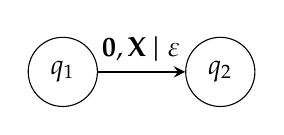
\begin{tikzpicture}[node distance = 2cm, on grid, auto]
    \node (q1) [state] {$q_1$};
    \node (q2) [state, right = of q1] {$q_2$};

    \path[-stealth, thick] (q1) edge node {$\mathbf{0,X \mid \varepsilon}$} (q2);
\end{tikzpicture}\\ \\
\end{center}
Tímto způsobem vyjadřujeme \textbf{ZA} velmi podobným způsobem jako \textbf{KA} stavovým diagramem.
\pagebreak
\section{Příklady}
\subsection*{Příklad 1}
Ukažme si návrh a diagram zásobníkového automatu, který akceptuje jazyk $\mathbf{L = \{a^nb^n \mid n \ge 0\}}$. V důkazu \textbf{pumping lemmatem} jsme dokázali, že \textbf{L} není regulární jazyk $\rightarrow$ nelze ho tedy vyjádřit s pomocí \textbf{KA}. Navrhněme tedy zásobníkový automat, který bude \textbf{L} generovat.\\ \\
Potřebovali bychom automat akceptující slova se stejným počtem znaků \textbf{a} a \textbf{b}. Logicky bychom tedy potřebovali nějak mít přehled o tom, jestli zrovna máme stejný počet těchto znaků, nebo ne. K tomu použijeme zásobník.\\ \\ Řekněme, že za každý zpracovaný znak \textbf{a} přidáme na zásobník \textbf{X}. Naopak za každý znak \textbf{b} na zásobník nepřidáme nic, ale přečteme z něho znak \textbf{X}. Takto zajistíme, že zpracované slovo \textbf{w} skončí s prázdným zásobníkem právě pokud $\mathbf{\mid{w}\mid_a{=}\mid{w}\mid_b}$.\\ \\
Pokud se při návrhu přechodů v našem automatu budeme řídit těmito pravidly, měli bychom vytvořit automat, který pro každé slovo tvaru $\mathbf{a^nb^n \mid n \ge 0}$ skončí průchod akceptováním. Ke generování jazyka \textbf{L} by nám měli stačit tři stavy.\\ \\
\begin{center}
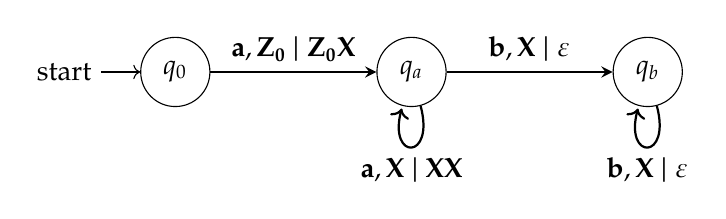
\begin{tikzpicture} [node distance = 3cm, on grid, auto]
   \node (q0)[state, initial] {$q_0$}; 
   \node (qa)[state, right = of q0] {$q_a$};
   \node (qb)[state, right = of qa] {$q_b$};

   \path[-stealth,thick](q0) edge node {$\mathbf{a,Z_0 \mid Z_0X}$}(qa);
   \path[-stealth,thick](qa) edge [loop below] node {$\mathbf{a,X \mid XX}$}(qa);
   \path[-stealth,thick](qa) edge node {$\mathbf{b,X \mid \varepsilon}$}(qb);
   \path[-stealth,thick](qb) edge [loop below] node {$\mathbf{b,X \mid \varepsilon}$}(qb);
\end{tikzpicture}
\end{center}
\\ \\(pozn. při zapisování na zásobník píšeme dva znaky, protože přečtením daný znak odstraňujeme)\\ \\
Tento automat by měl generovat jazyk \textbf{L}. Zároveň jsme ho navrhli tak, že akceptuje pouze slova, kde první je sekvence znaků \textbf{a}, pak \textbf{b}. Jakmile v libovolném stavu nastane situace, že slovo je zpracované a zásobník prázdný $\rightarrow$ slovo je akceptované.
\pagebreak
\\ \\
Popišme si průběh zpracování několika slov:
\vspace{0.4cm}    
\hrule
\vspace{0.1cm}
\begin{description}
    \item[\fbox{$\mathbf{w = aaabbb}$}] Zpracování slova začíná ve stavu $\mathbf{q_0}$ a s prázdným zásobníkem. Máme tedy $\mathbf{(q_0,aaabbb,Z_0)\rightarrow (q_a,aabbb,Z_0X)}$. Nyní jsme ve stavu $\mathbf{q_a}$, na zásobníku je \textbf{X} a na vstupu \textbf{a}. Tudíž budeme teď procházet smyčkou ve stavu $\mathbf{q_a}$, dokud nenarazíme na znak \textbf{b}.\\ \\Tedy $\mathbf{(q_a,aabbb,Z_0X)\rightarrow(q_a,abbb,Z_0XX)\rightarrow(q_a,bbb,Z_0XXX)}$. \\ Nyní máme na vstupu znak \textbf{b} a na zásobníku \textbf{X}, tedy přecházíme do dalšího stavu \\ 
    $\mathbf{(q_a,bbb,Z_0XXX) \rightarrow (q_b,bb,Z_0XX)\rightarrow(q_b,b,Z_0X)\rightarrow(q_b,\varepsilon,Z_0)}$. Tím jsme se dostali do akceptujícího stavu, tudíž slovo je \textbf{akceptované}.
    
    \item[\fbox{$\mathbf{w = \varepsilon}$}] Tento příklad je jednoduchý, neboť již na začátku jsme v akceptujícím stavu $\mathbf{(q_0,\varepsilon,Z_0)}$.
    
    \item[\fbox{$\mathbf{w = abb}$}] Začínáme $\mathbf{(q_0,abb,Z_0)\rightarrow(q_a,bb,Z_0X)\rightarrow(q_b,b,Z_0)}$. Zde jsme ale skončili, protože nemáme definovaný přechod ze stavu $\mathbf{q_b}$, pokud čteme znak \textbf{b} a zásobník \textbf{není} prázdný. To znamená, že toto slovo nemá stejný počet znaků \textbf{a} a \textbf{b} $\rightarrow$ automat ho \textbf{neakceptuje}.
\end{description}
\vspace{0.1cm}    
\hrule
\vspace{0.4cm}
Vidíme tedy, že automat pracuje tak, jak bychom chtěli.
\pagebreak
\\ \\
\subsection*{Příklad 2}
Ukažme si ještě jeden automat podobný tomu předchozímu. Navrhněme \textbf{ZA} generující jazyk $\mathbf{J = \{w\in\{a,b\}^* ; \mid{w}\mid_a=\mid{w}\mid_b\}}$, neboli jazyk slov se stejným počtem znaků \textbf{a} jako \textbf{b}. Rozdíl od předešlého příkladu je ten, že nám nezáleží na pořadí znaků ani na tom, jak se budou střídat. Zajímá nás čistě jen jejich počet.\\ \\
Zásobník bude v tomto automatu fungovat podobně jako v minulém příkladu. Je ale třeba si uvědomit, že musíme počítat výskyt zrovna toho znaku, kterého je v daný moment víc. Například řetězec \textbf{aaabbbba} patří do \textbf{J}, ale pokud by zásobník fungoval stejně jako v minulém příkladě, automat by slovo neakceptoval. Budeme tedy muset přechody navrhnout tak, abychom přidávali na zásobník \textbf{X} za zrovna častější znak a odebírali za druhý.\\ \\
V praxi může automat generující \textbf{J} navrhnout třeba takto:\\ \\
\begin{center}
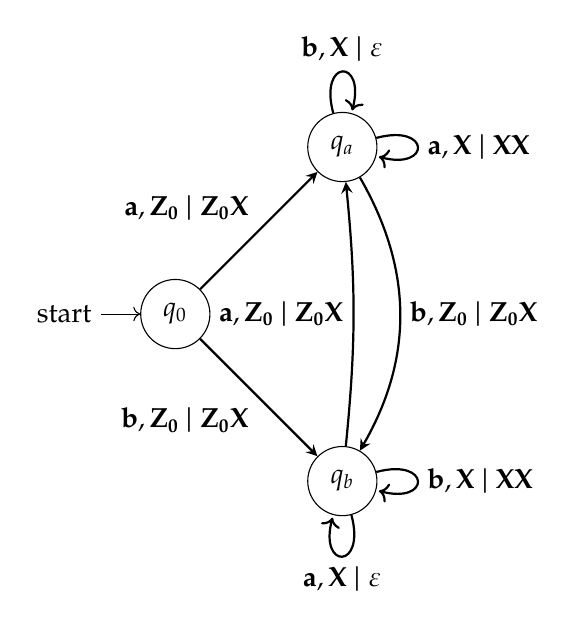
\begin{tikzpicture} [node distance = 3cm, on grid, auto]
   \node (q0)[state, initial] {$q_0$}; 
   \node (qa)[state, above right = of q0] {$q_a$};
   \node (qb)[state, below right = of q0] {$q_b$};

   \path[-stealth, thick](q0)edge node{$\mathbf{a,Z_0 \mid Z_0X}$}(qa);
   \path[-stealth, thick](q0)edge node[below left]{$\mathbf{b,Z_0 \mid Z_0X}$}(qb);
   \path[-stealth, thick](qa)edge [loop right] node{$\mathbf{a,X \mid XX}$}(qa);
   \path[-stealth, thick](qb)edge [loop right]node{$\mathbf{b,X \mid XX}$}(qb);
   \path[-stealth, thick](qb)edge [loop below]node{$\mathbf{a,X \mid \varepsilon}$}(qb);
   \path[-stealth, thick](qa)edge [loop above]node{$\mathbf{b,X \mid \varepsilon}$}(qa);
   \path[-stealth, thick](qa)edge [bend left] node{$\mathbf{b,Z_0 \mid Z_0X}$}(qb);
   \path[-stealth, thick](qb)edge [bend right = 0.2cm] node{$\mathbf{a,Z_0 \mid Z_0X}$}(qa);
\end{tikzpicture}\\ \\
\end{center}
Tento automat v závislosti na prvním znaku slova přejde do $\mathbf{q_a}$ nebo $\mathbf{q_b \rightarrow}$ za tento znak začne přidávat na zásobník \textbf{X} a za druhý znak odebírat \textbf{X}. Pokud se znaky vyrovnají (zásobník se vyprázdní) a začne převládat druhý znak, automat přejde do jeho stavu a začne přidávat \textbf{X} za něj.\\ \\
Podívejme se na již zmíněné slovo \textbf{aaabbbba}. \textbf{ZA} ho zpracuje následovně:\\ \\
$\mathbf{(q_0,aaabbbba,Z_0)\rightarrow(q_a,aabbbba,Z_0X)\rightarrow(q_a,abbbba,Z_0XX)\rightarrow}$\\$\mathbf{(q_a,bbbba,Z_0XXX)\rightarrow(q_a,bbba,Z_0XX)\rightarrow ... \rightarrow (q_a,ba,Z_0)\rightarrow}$\\$\mathbf{(q_b,a,Z_0X)\rightarrow(q_b,\varepsilon,Z_0)\rightarrow}$ \textbf{akceptuje}
\setcounter{chapter}{6}
\setcounter{section}{0}
\chapter*{Turingův stroj}
\addcontentsline{toc}{chapter}{Turingův stroj}
Turingův stroj je zásadním nástrojem v oboru informatiky a matematiky. Jedná se o stroj nacházející se na vrcholu hierarchie abstraktních výpočetních modelů, což ho staví nad již probrané \textbf{konečné a zásobníkové automaty}. Turingův stroj je totiž model schopný simulovat jakýkoliv jiný algoritmický proces. Jinými slovy je schopen se chovat jako \textbf{KA}, \textbf{ZA}, nebo jako jakýkoliv jiný model řešící nějaký problém. Automaty definované v předchozích kapitolách jsou pouze zjednodušenými specifickými verzemi \textbf{Turingova stroje}.
\section{Turingův stroj}
\subsection*{Definice}
Před formální definicí si \textbf{Turingův stroj} definujeme trochu abstraktně, čímž lépe pochopíme jeho jednotlivé složky.\\ \\
Představme si Turingův stroj jako dva předměty - \textbf{Stroj se čtecí hlavou} a \textbf{nekonečnou vstupní pásku}. Stroj má několik vnitřních stavů, mezi kterými přechází v závislosti na aktuálním stavu a znacích čtených z pásky. Čtecí hlava stroje může vždy přečíst jen jeden znak z pásky a \textbf{může se po ní pohybovat v obou směrech}. Stroj také může znak čtený na pásce přepsat na jiný.\\ \\
Pokud správně dodefinujeme vnitřní stavy stroje a to, za jakých podmínek bude stroj stavy měnit, jsme schopni simulovat jakýkoliv algoritmický proces. Nyní si \textbf{TS} zadefinujeme formálně:\\ \\
\textbf{Turingův stroj} je definován šesticí $\mathbf{M=\{Q,\Gamma,\Sigma,\delta,q_0,F\}}$, kde:
\vspace{0.4cm}    
\hrule
\vspace{0.1cm}
    \begin{description}
        \item[\fbox{Q}] Konečná neprázdná množina stavů
        \item[\fbox{$\mathbf{\Gamma}$}] Pásková abeceda
        \item[\fbox{$\mathbf{\Sigma}$}] Vstupní abeceda, obecně platí $\mathbf{\Sigma = \Gamma \backslash \{b\}}$, kde \textbf{b} je prázdný (\textbf{blank}) znak
        \item[\fbox{$\mathbf{\delta}$}] Přechodová funkce $\mathbf{(Q\backslash{F}) \times \Gamma \rightarrow Q \times \Gamma \times \{-,0,+\}}$, neboli funkce, která v závislosti na přečteném nekoncovém stavu $q_a$ a znaku $x$ na pásce přejde do $q_b$, případně změní $x$ na pásce a/nebo se posune.\\ \\(pozn: \textbf{-} doleva, \textbf{0} nic, \textbf{+} doprava)
        \item[\fbox{$\mathbf{q_0}$}] Počáteční stav, platí $\mathbf{q_0 \in Q}$
        \item[\fbox{F}] množina koncových stavů, platí $\mathbf{F \subseteq Q}$. Pokud se \textbf{TS} dostane zpracováním slova \textbf{w} na vstupní pásce do stavu $q \in \mathbf{F}$, pak \textbf{TS} slovo \textbf{w} akceptuje.\\ \\
        Nekonečná zpracování pak \textbf{TS} neakceptuje. Často také pro \textbf{TS} definujeme koncové stavy $q_{acc}$ a $q_{rej}$, přičemž zpracování končící v $q_{acc}$ akceptuje a ty v $q_{rej}$ ne.
    \end{description}
\vspace{0.1cm}    
\hrule
\vspace{0.4cm}  
Slova ke zpracování \textbf{TS} tedy klademe na nekonečnou pásku, přičemž všechno 'nevyužité' místo na pásce zaplníme prázdným znakem \textbf{b}.\\ \\
Slovo zapsané na pásku a pozice čtecí hlavy \textbf{TS} definujeme jako jeho \textbf{počáteční konfiguraci}.\\ \\
Krok \textbf{TS} budeme vnímat asi takto: Pokud \textbf{TS} je ve stavu $q_a$ a přečte znak \textbf{x} z pásky, přejde do stavu $q_b$, místo \textbf{x} vepíše na pásku \textbf{x'} a posune se po pásce o $\mathbf{d \in \{-,0,+\}}$. Je důležité si uvědomit, že se nemusí posunout, nic přepsat ani přejít do jiného stavu (tedy $q_a=q_b,\mathbf{x=x'},\mathbf{d=0}$). Notace jednoho kroku \textbf{TS} tedy je \fbox{$\mathbf{\delta(q_a,x) \rightarrow (q_b,x',d)}$}.\\ \\
Také je důležité si uvědomit, že pokud při úspěšném zpracování slova \textbf{w} dojde k jeho změně automatem, do generovaného jazyka přidáváme původní slovo \textbf{w}.\\ \\
Ačkoliv takto se může zdát definice \textbf{TS} zmatečná, v praxi s ním pracujeme velmi podobně jako s \textbf{KA} nebo \textbf{ZA}, což si ukážeme v následujících sekcích.
\section{Graf TS}
Stejně jako \textbf{KA} nebo \textbf{ZA}, i \textbf{Turingův stroj} vyjadřujeme nejčastěji v grafické podobě stavového diagramu či grafu. V této podobě jsou pak jednotlivé stavy stroje vyobrazené jako stavy grafu. Hrany mezi stavy budou popisovat pravidla definovaná přechodovou funkcí. Představme si tedy situaci, kdy jsme ve stavu $q_a$, čteme \textbf{x}, máme zapsat \textbf{y}, přesunout se po pásce o znak vpřed a přejít do stavu $q_b$ (neboli $\mathbf{\delta(q_a,x) \rightarrow (q_b,y,+)}$). Tento krok vyobrazíme následovně:\\ \\
\begin{center}
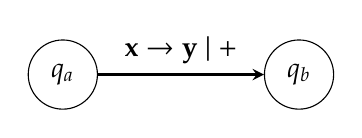
\begin{tikzpicture} [node distance = 3cm, on grid, auto]
   \node (qa)[state] {$q_a$};
   \node (qb)[state, right = of qa] {$q_b$};

   \path[-stealth,thick](qa) edge node {$\mathbf{x \rightarrow y \mid +}$}(qb);

\end{tikzpicture}\\ \\
\end{center}
Tímto způsobem jsme schopni popsat stavy stroje a přechodové funkce, které je spojují.
\section{Příklad}
Zkusme si navrhnout \textbf{TS}, který zadané slovo \textbf{w} nad abecedou $\mathbf{\{0, 1\}}$ invertuje, neboli převede $\mathbf{0 \rightarrow 1 , 1 \rightarrow 0}$. Nechť náš \textbf{TS} začíná zpracování s čtecí hlavou na prvním znaku zleva.\\ \\ Jako první je dobré si projít, čeho chceme dosáhnout a jaké situace nás mohou potkat. Jelikož má naše abeceda pouze 2 znaky, které se invertují jeden na druhý, bude to celkem snadné. Existují pouze 3 znaky, které může naše hlava přečíst:
\begin{description}
        \item[\fbox{0}] Chceme přepsat na \textbf{1}
        \item[\fbox{1}] Chceme přepsat na \textbf{0}
        \item[\fbox{b}] Prázdný znak
    \end{description}
Z tohoto je snad vidět, že musíme definovat aspoň 2 přechodové funkce - jednu pro invertování $\mathbf{0 \rightarrow 1}$, druhou pro invertování  $\mathbf{1 \rightarrow 0}$. Jinak se ve splnění zadání neposuneme.\\ \\ Jelikož počáteční konfigurace hlavy je na prvním znaku vlevo, můžeme si uvědomit, že nám bude stačit postupovat pouze vpravo slovem a '\textit{invertovat}' jednotlivé znaky.\\ \\Poslední věc, kterou si musíme uvědomit, je konec zpracování slova. Asi je jasné, že všechna slova $\mathbf{w \in \{0, 1\}^{*}}$ lze invertovat. Tedy každé zpracování skončí v nějakém akceptujícím koncovém stavu $q_{acc}$. Logicky bychom se do něj měli dostat jen poté, co jsme invertovali celé slovo \textbf{w}. To nastane tehdy, když se čtecí hlava dostane na první prázdný znak \textbf{b} vpravo od slova (za předpokladu, že se budeme posouvat pouze doprava, jak jsme si stanovili).\\ \\Pokud spojíme tyto naše poznatky dohromady, jsme schopni navrhnout \textbf{TS}. Definujme si tedy 2 stavy $\mathbf{\{q_{inv}, q_{acc}\}}$. Stav $\mathbf{q_{inv}}$ bude náš počáteční a zároveň '\textit{pracující}' stav. Pokud se v něm nacházíme a čteme nějaký znak slova \textbf{w}, tak ho invertujeme, posuneme se o jeden znak doprava a zůstáváme v $\mathbf{q_{inv}}$. Jinými slovy definujeme $\mathbf{\delta(q_{inv},0) \rightarrow (q_{inv},1,+)}$ a $\mathbf{\delta(q_{inv},1) \rightarrow (q_{inv},0,+)}$. Musíme také definovat konec zpracování slova, neboli přechod do $\mathbf{q_{acc}}$. Ten nastane, pokud jsme zpracovali celé slovo, neboli pokud čteme znak \textbf{b}. Tedy definujeme $\mathbf{\delta(q_{inv},b) \rightarrow (q_{acc},b,+)}$.
\pagebreak
\\ \\Tímto jsme skončili. Pokud si nyní nakreslíme to, co jsme definovali, získáme:\\ \\
\begin{center}
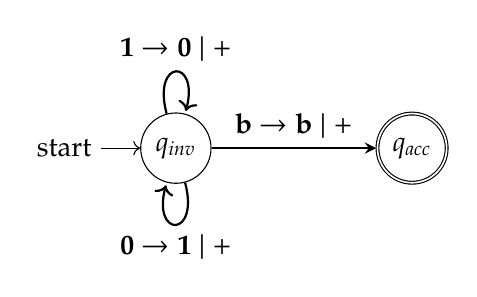
\begin{tikzpicture} [node distance = 3cm, on grid, auto]
   \node (qa)[state,initial] {$q_{inv}$};
   \node (qb)[state, right = of qa,accepting] {$q_{acc}$};

   \path[-stealth,thick](qa) edge [loop below] node {$\mathbf{0 \rightarrow 1 \mid +}$}(qa);
   \path[-stealth,thick](qa) edge [loop above] node {$\mathbf{1 \rightarrow 0 \mid +}$}(qa);
   \path[-stealth,thick](qa) edge node {$\mathbf{b \rightarrow b \mid +}$}(qb);
    

\end{tikzpicture}\\ \\
\end{center}
Zkusme si napsat postup pro slovo $\mathbf{w = 0110}$:\\ \\
\begin{enumerate}
    \item $\mathbf{\delta(q_{inv},0) \rightarrow (q_{inv},1,+) \mid 0110 \rightarrow 1110}$
    \item $\mathbf{\delta(q_{inv},1) \rightarrow (q_{inv},0,+) \mid 1110 \rightarrow 1010}$ 
    \item $\mathbf{\delta(q_{inv},1) \rightarrow (q_{inv},0,+) \mid 1010 \rightarrow 1000}$ 
    \item $\mathbf{\delta(q_{inv},0) \rightarrow (q_{inv},1,+) \mid 1000 \rightarrow 1001}$
    \item $\mathbf{\delta(q_{inv},b) \rightarrow (q_{acc},b,+) \mid 1001}$ 
\end{enumerate}
Snad je z tohoto popisu běh \textbf{TS} zřejmý.
\chapter*{Zajímavé zdroje a odkazy}
Následuje výpis odkazů na různé internetové zdroje, které nám sloužili jako inspirace. V případě nejasností v tomto textu či zvídavosti čtenáře doporučujeme relevantní zdroj navštívit:



\vspace{0.4cm}    
\hrule
\vspace{0.1cm}
  \begin{itemize}
      \item[]https://www.cs.vsb.cz/sawa/uti/2021/slides/uti-02-cz.pdf
      \item[]https://www.cs.vsb.cz/sawa/uti/materialy/uti.pdf
      \item[]https://www.cs.vsb.cz/sawa/uti/2020/slides/uti-07-cz.pdf
      \item[]https://www.youtube.com/watch?v=47awv0bU3Hc
      \item[]https://www.youtube.com/watch?v=C5KerRqrC8c
      \item[]https://www.youtube.com/watch?v=WpdhNNtYMJY
      \item[]https://youtu.be/uzFVAmk3uXc?si=\_1bOM0sAgmmqIZHv
      \item[]https://www.youtube.com/watch?v=8Defwmq5X5E
      \item[]https://youtu.be/uzFVAmk3uXc?si=cwy9RR9Z8F2nBCYU
      \item[]https://youtu.be/QAacOfpV5GY?si=-hJniGDLQQDMJnGd
      \item[]https://youtu.be/Y7FZdvqISDU?si=EkUb7p-ZF\_zhAdfI 
      \item[]https://youtu.be/kFx0FnPaRF8?si=yzkMGPpEmHik\_sNp 
      \item[]https://www.youtube.com/watch?v=6YCrUSMdwbk
      \item[]https://www.youtube.com/watch?v=YQDfJmKLKsc 
      \item[]https://youtu.be/MMFBhaWeUDY?si=6ajzGvw1JzaqWdZh
      \item[]https://youtu.be/yCaweOE8VIo?si=Yhp68i8bTmaKoSYc 
      \item[]https://youtu.be/44se2RSyXx0?si=O7K6hSC0zeXmWfYh
      \item[] https://youtu.be/4uVAwwjQnJk?si=5a4abUFn4HwKo83X
      
  \end{itemize}
\vspace{0.1cm}    
\hrule
\vspace{0.4cm}  

\end{document}
